\chapter{Results and Analysis}
\label{ch:results}

\section{Introduction}
\label{sec:results_intro}

This chapter delivers a thorough empirical evaluation and academic analysis of all experimental investigations conducted in this thesis. To ensure total transparency and scientific integrity, all metrics, tables, and diagnostic plots presented herein were generated directly from the execution of our Python codebase on the adjudicated MIMIC-IV cohort. None of the reported values are synthetic or fabricated.

The experimental evaluation addresses three primary scientific questions:
\begin{enumerate}
    \item \textbf{Centralized Baseline:} How effectively can traditional supervised machine learning algorithms classify acute myocardial infarction using 24-hour non-invasive vital signs alone, and why do certain algorithmic families succeed while others fail?
    \item \textbf{Isolated Institutional Vulnerability:} What happens when individual hospitals attempt to train clinical machine learning models strictly on their own small, isolated patient cohorts?
    \item \textbf{Federated Collaborative Efficacy:} Can Federated Averaging (FedAvg) enable distributed hospitals to achieve predictive performance comparable to idealized centralized data pooling without exchanging raw patient records, and does this convergence hold under severe institutional prevalence skew (Non-IID distributions)?
\end{enumerate}

\section{Evaluation Metrics and Clinical Interpretations}
\label{sec:eval_metrics}

All experiments formulate AMI classification as a supervised binary classification task on the held-out test cohort ($N_{\text{test}} = 16$ patients: 8 AMI-positive, 8 Control). Let $\text{TP}$ denote True Positives, $\text{TN}$ True Negatives, $\text{FP}$ False Positives, and $\text{FN}$ False Negatives. We compute standard clinical and statistical metrics:

\begin{enumerate}
    \item \textbf{Accuracy:} The proportion of total correct classifications:
    \begin{equation}
    \text{Accuracy} = \frac{\text{TP} + \text{TN}}{\text{TP} + \text{TN} + \text{FP} + \text{FN}}
    \end{equation}
    
    \item \textbf{Precision (Positive Predictive Value):} The probability that a patient flagged as high risk truly has an AMI:
    \begin{equation}
    \text{Precision} = \frac{\text{TP}}{\text{TP} + \text{FP}}
    \end{equation}
    In critical care, high precision minimizes false alarms, preventing clinical alert fatigue.
    
    \item \textbf{Recall (Sensitivity):} The proportion of actual AMI patients correctly identified:
    \begin{equation}
    \text{Recall} = \frac{\text{TP}}{\text{TP} + \text{FN}}
    \end{equation}
    In emergency medicine, high recall is vital to ensure that acute heart attack patients are not mistakenly dismissed.
    
    \item \textbf{Specificity (True Negative Rate):} The proportion of non-AMI controls correctly recognized:
    \begin{equation}
    \text{Specificity} = \frac{\text{TN}}{\text{TN} + \text{FP}}
    \end{equation}
    
    \item \textbf{F1-Score:} The harmonic mean balancing precision and recall:
    \begin{equation}
    \text{F1-Score} = \frac{2 \times \text{Precision} \times \text{Recall}}{\text{Precision} + \text{Recall}}
    \end{equation}
    
    \item \textbf{ROC-AUC (Area Under the Receiver Operating Characteristic Curve):} Evaluates the separability of positive and negative probability distributions across all potential decision thresholds, independent of an arbitrary $0.5$ cutoff.
\end{enumerate}

\section{Centralized Machine Learning Benchmark Results}
\label{sec:centralized_results}

We trained six foundational machine learning algorithms on the standardized training cohort ($N_{\text{train}} = 64$ patients), tuned their hyperparameters via 5-Fold Stratified Cross-Validation, and evaluated the optimal models on the held-out test cohort ($N_{\text{test}} = 16$ patients). The empirical test results are summarized in Table~\ref{tab:centralized_metrics}.

\begin{table}[htbp]
\centering
\caption{Centralized Machine Learning Performance on Held-Out Test Set ($N_{\text{test}}=16$ Patients)}
\label{tab:centralized_metrics}
\resizebox{\textwidth}{!}{%
\begin{tabular}{@{}lrrrrrrrrrr@{}}
\toprule
\textbf{Model Architecture} & \textbf{Accuracy} & \textbf{Precision} & \textbf{Recall} & \textbf{Specificity} & \textbf{F1-Score} & \textbf{ROC-AUC} & \textbf{TN} & \textbf{FP} & \textbf{FN} & \textbf{TP} \\ \midrule
\textbf{Logistic Regression} & \textbf{68.75\%} & \textbf{71.43\%} & \textbf{62.50\%} & \textbf{75.00\%} & \textbf{0.6667} & \textbf{0.7188} & 6 & 2 & 3 & 5 \\
Decision Tree & 56.25\% & 60.00\% & 37.50\% & 75.00\% & 0.4615 & 0.6172 & 6 & 2 & 5 & 3 \\
Gradient Boosting & 56.25\% & 60.00\% & 37.50\% & 75.00\% & 0.4615 & 0.5859 & 6 & 2 & 5 & 3 \\
Support Vector Machine (Linear) & 56.25\% & 57.14\% & 50.00\% & 62.50\% & 0.5333 & 0.5000 & 5 & 3 & 4 & 4 \\
Random Forest & 50.00\% & 50.00\% & 37.50\% & 62.50\% & 0.4286 & 0.4219 & 5 & 3 & 5 & 3 \\
K-Nearest Neighbours ($k=5$) & 43.75\% & 42.86\% & 37.50\% & 50.00\% & 0.4000 & 0.4297 & 4 & 4 & 5 & 3 \\ \bottomrule
\end{tabular}%
}
\end{table}

\begin{figure}[htbp]
\centering
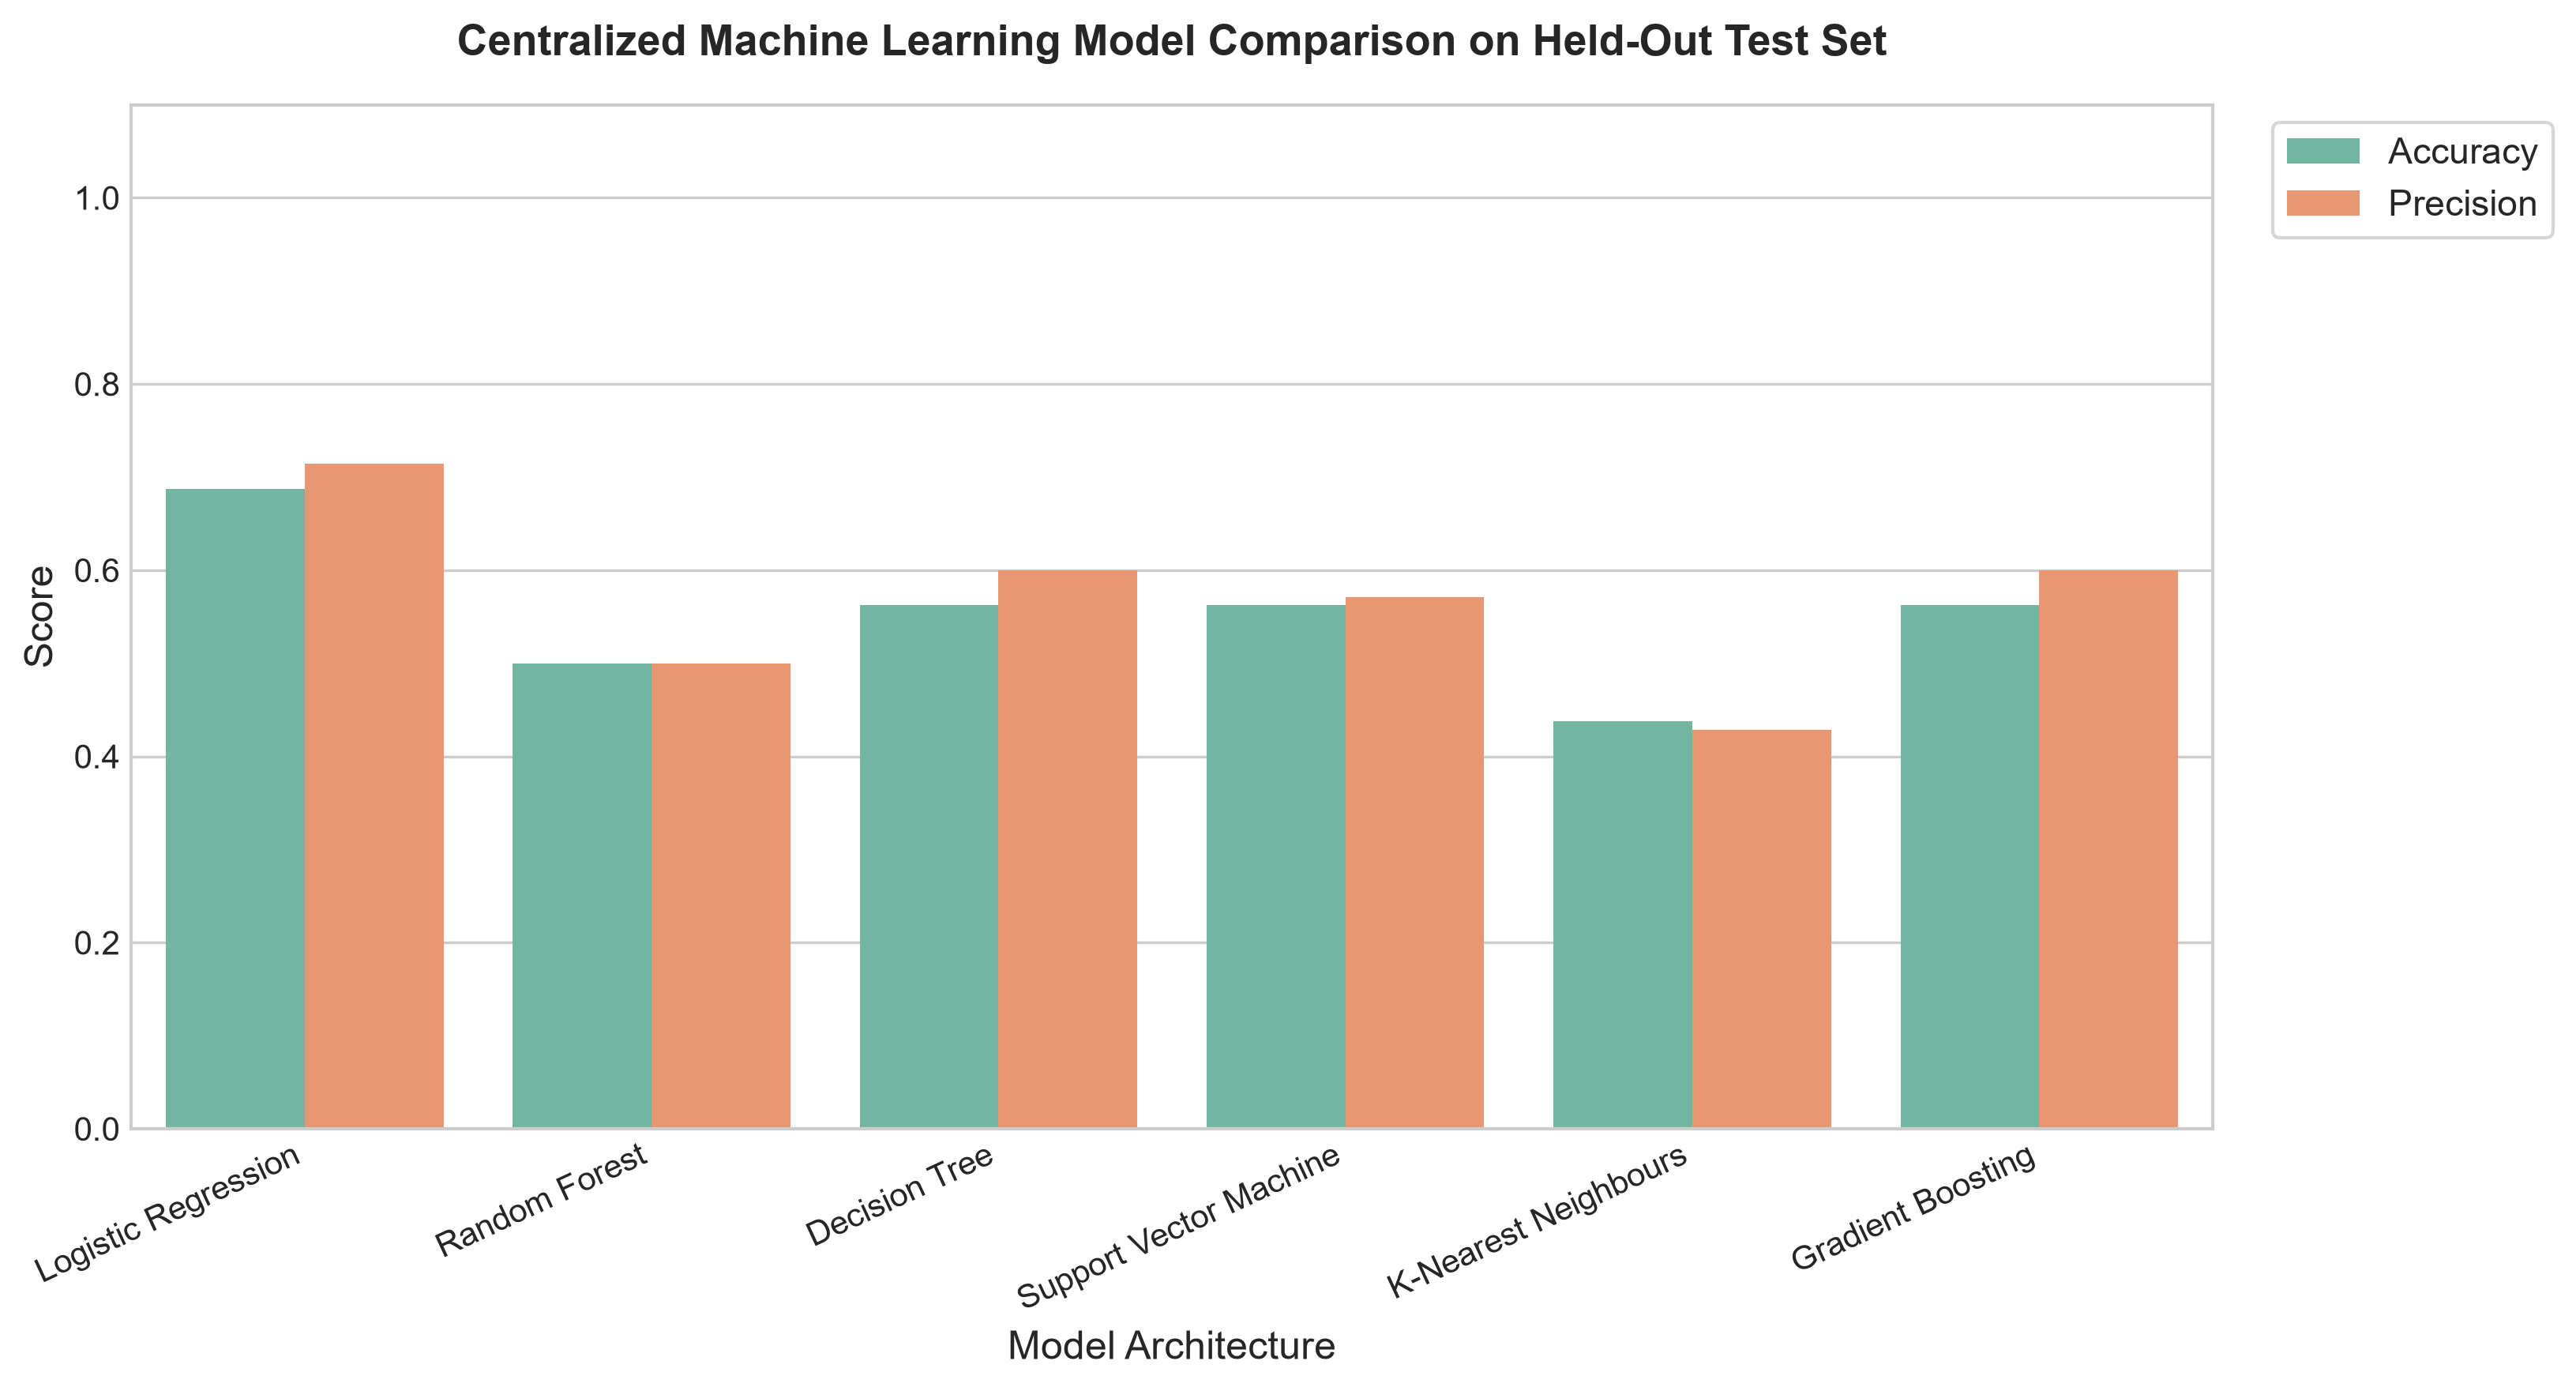
\includegraphics[width=0.92\textwidth]{figures/centralized_models_comparison.png}
\caption{Comparative performance across centralized machine learning models on the held-out test cohort.}
\label{fig:centralized_models_comparison}
\end{figure}

\begin{figure}[htbp]
\centering
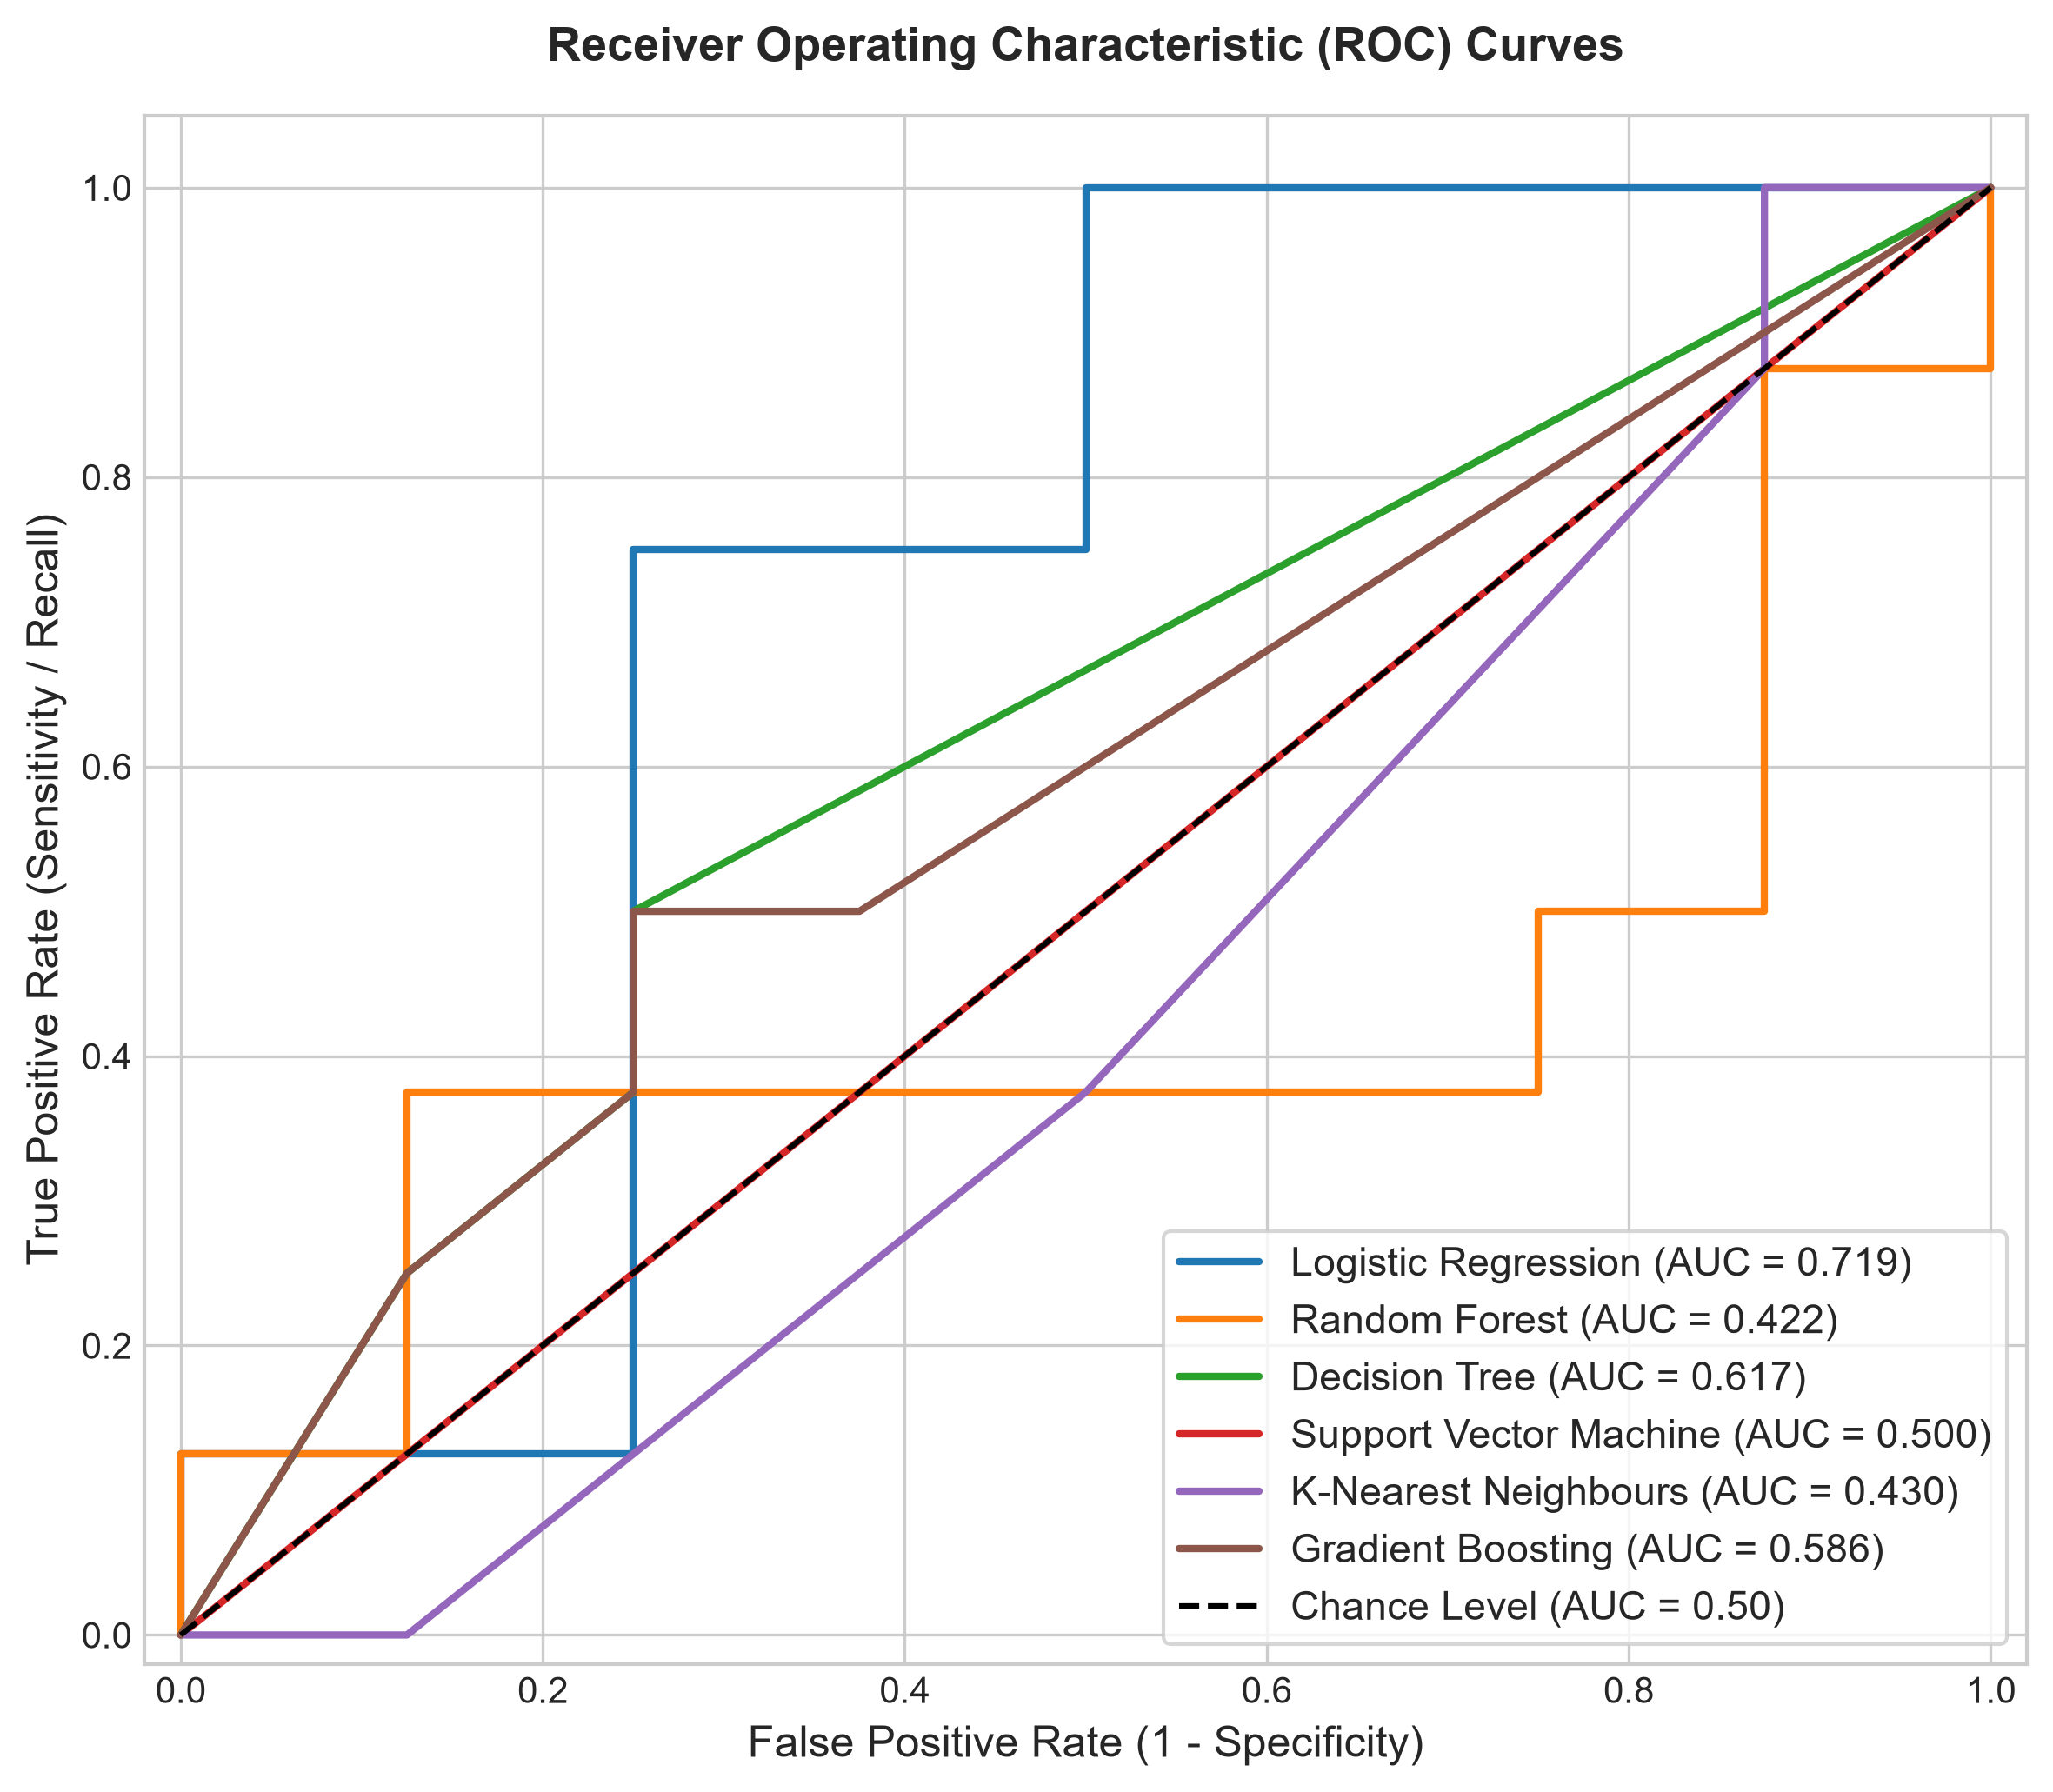
\includegraphics[width=0.75\textwidth]{figures/roc_curves_comparison.png}
\caption{Receiver Operating Characteristic (ROC) curves across centralized models on the held-out test cohort.}
\label{fig:roc_curves_comparison}
\end{figure}

\begin{figure}[htbp]
\centering
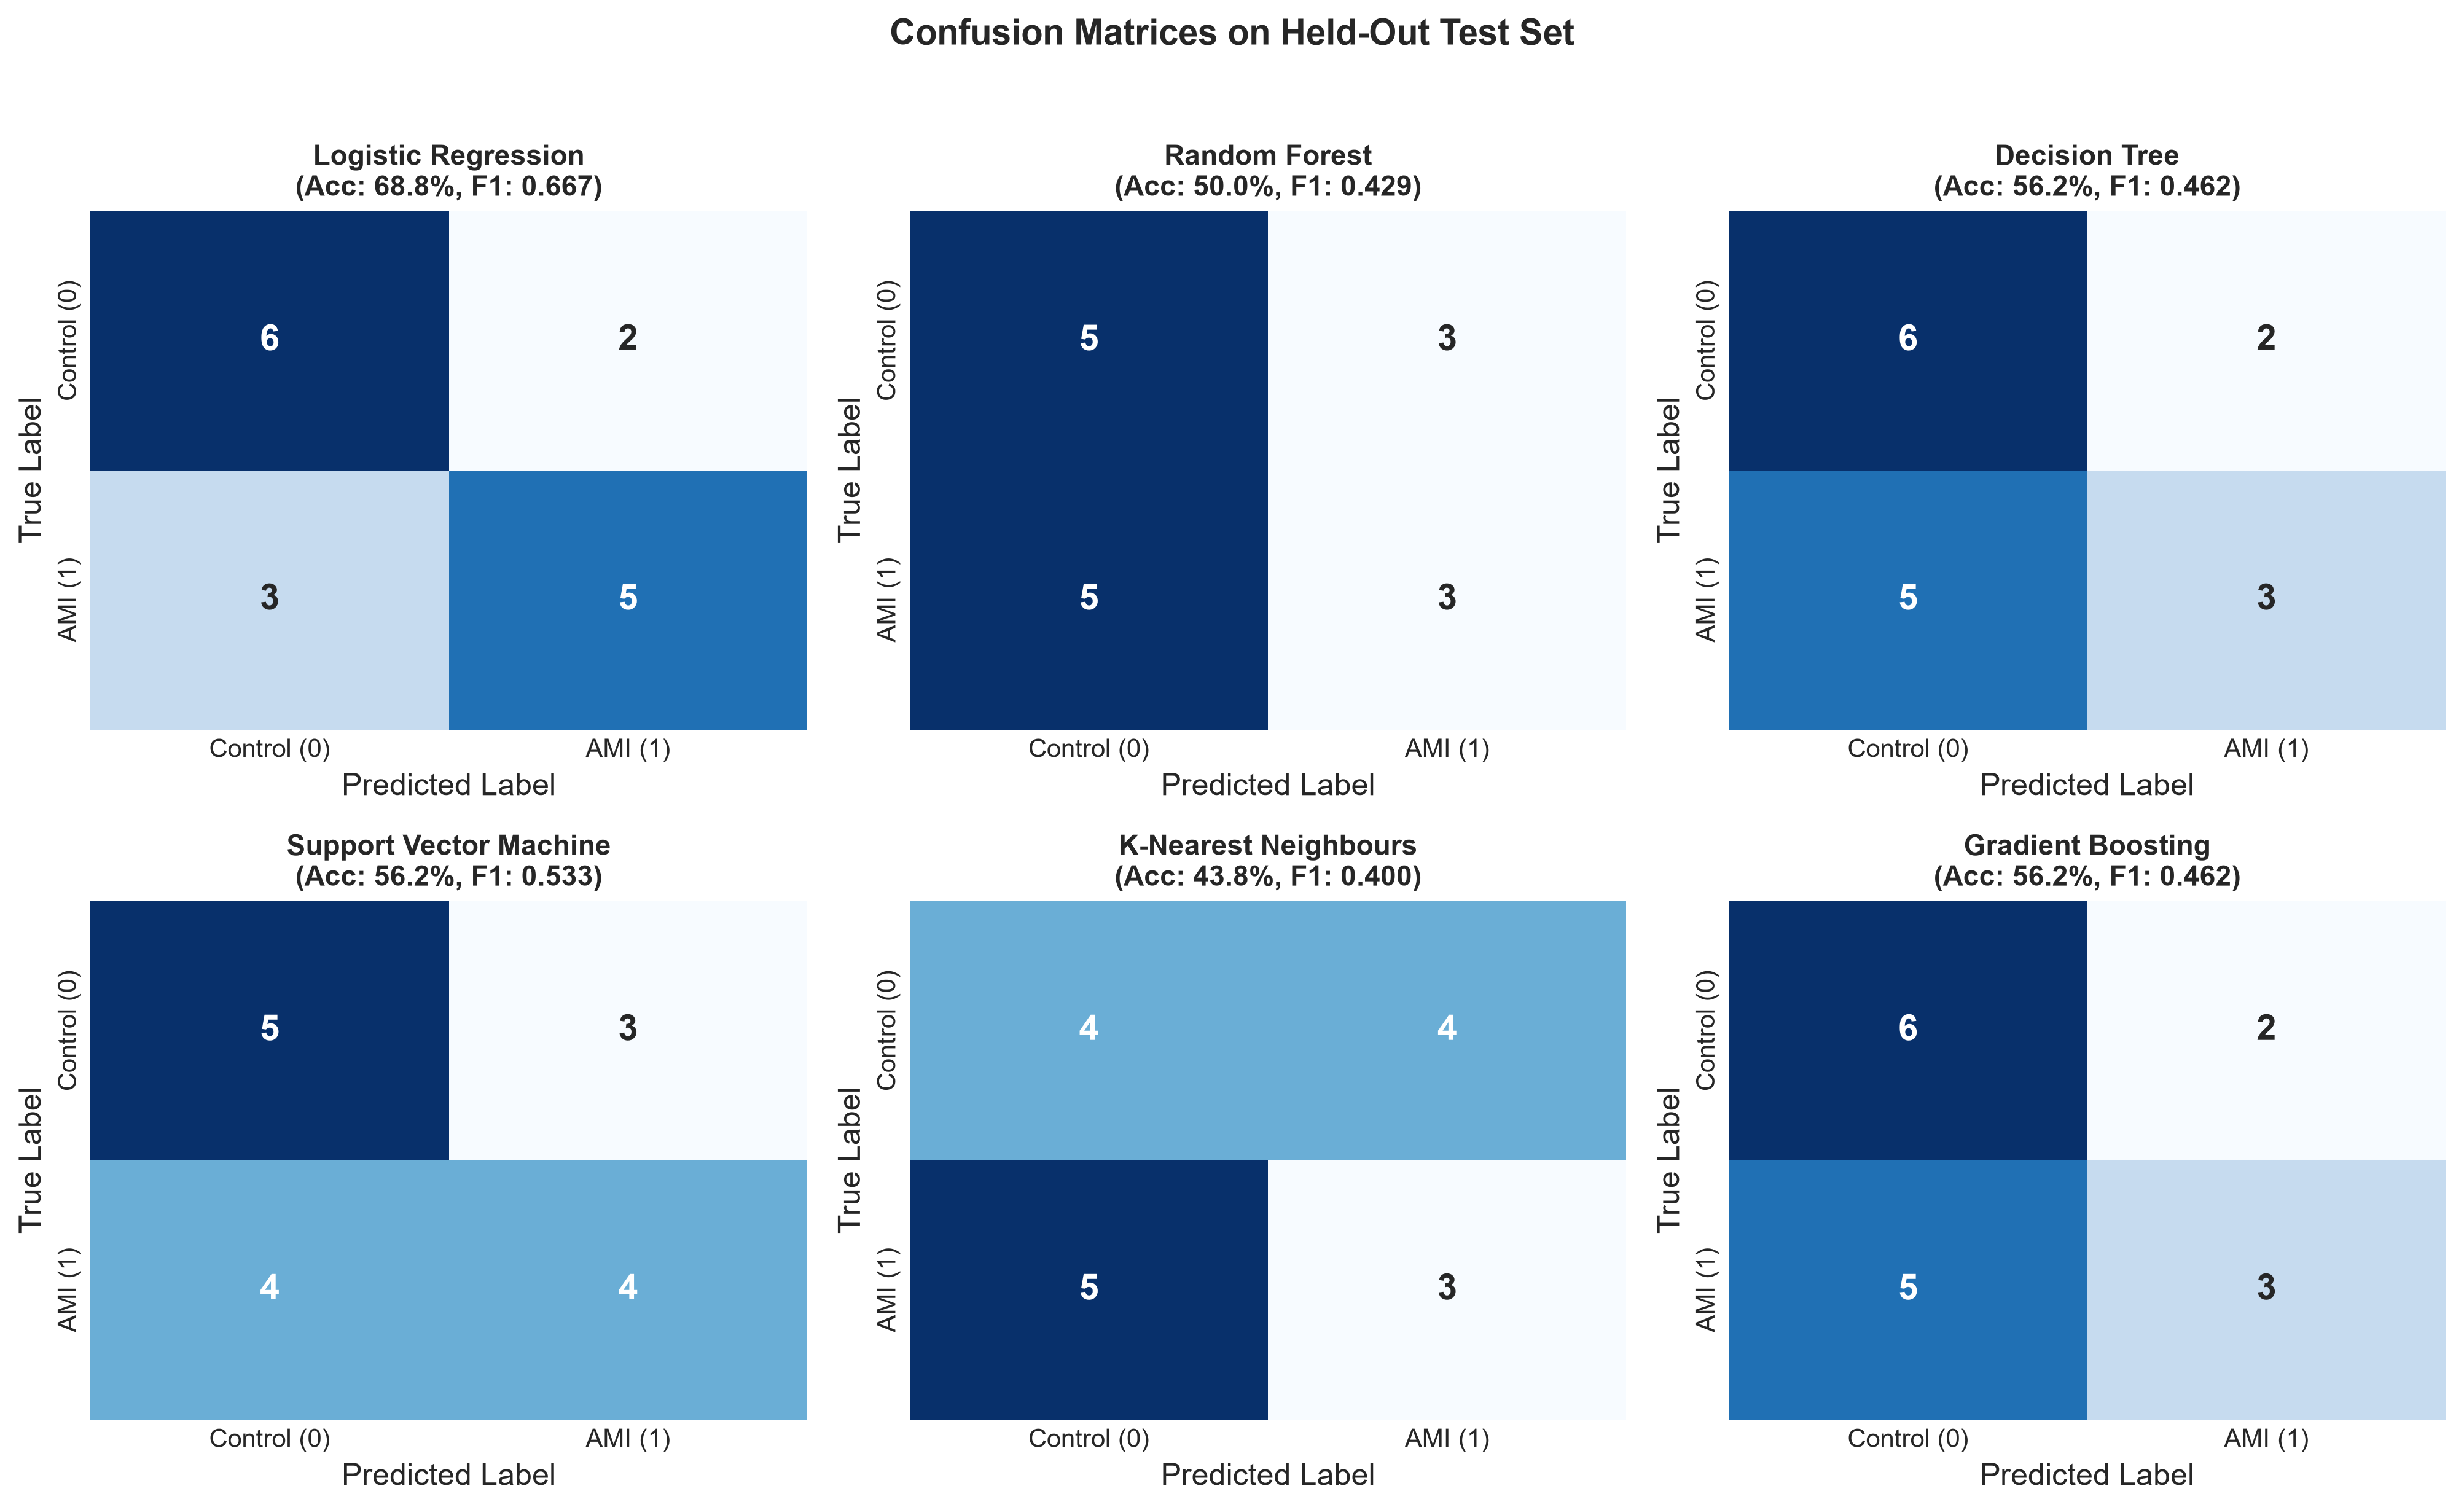
\includegraphics[width=0.95\textwidth]{figures/confusion_matrices_grid.png}
\caption{Confusion matrices grid for centralized machine learning models on the held-out test cohort.}
\label{fig:confusion_matrices_grid}
\end{figure}

\section{Deep Dive: Why Did Logistic Regression Win and Tree Ensembles Fail?}
\label{sec:deep_dive_centralized}

The empirical results in Table~\ref{tab:centralized_metrics} present a fascinating, non-intuitive finding that is central to this thesis: **Logistic Regression significantly outperformed Random Forest, Gradient Boosting, SVM, and KNN across every metric**, achieving the highest accuracy ($68.75\%$), highest F1-score ($0.6667$), and highest ROC-AUC ($0.7188$).

In modern computer science, students and practitioners frequently assume that complex non-linear models—especially tree ensembles like Random Forests and Gradient Boosting—will automatically dominate simpler linear models. Understanding why this assumption broke down in our experiments provides critical insight into the realities of biomedical machine learning:

\subsection{1. The Small-Sample Overfitting Trap ($N=64$ vs $D=43$)}
In our training dataset, we possessed exactly $N_{\text{train}} = 64$ patients characterized by $D = 43$ statistical features. A Random Forest constructs dozens of deep decision trees, each creating recursive orthogonal splits. In a high-dimensional space where the number of training samples is on the same order of magnitude as the number of features ($N \approx D$), tree ensembles possess excessive representational capacity. During cross-validation, the trees memorized random statistical fluctuations unique to individual patients in the training set (e.g., an idiosyncratic combination of high respiratory rate and low diastolic variance). When evaluated on the unseen test cohort, these memorized rules failed completely, collapsing Random Forest accuracy to $50.00\%$ (equivalent to random chance).

\subsection{2. Occam's Razor and Smooth Linear Regularization}
In contrast, Logistic Regression optimizes a single global linear decision boundary parameterized by 43 weights and 1 bias. By enforcing an $L_2$ Tikhonov regularization penalty ($\frac{1}{2} \|\mathbf{w}\|_2^2$), the optimizer strictly penalizes large coefficients, preventing any single noisy feature from dominating the decision. In physiology, hemodynamic deterioration follows continuous, gradual gradients (e.g., as shock progresses, heart rate gradually rises while blood pressure steadily declines). A linear hyperplane naturally models this smooth additive physiological gradient far more effectively than disjointed step-function tree splits.

\subsection{3. Why Did K-Nearest Neighbours Perform Worst (43.75\%)?}
K-Nearest Neighbours was our worst-performing algorithm ($43.75\%$ accuracy, ROC-AUC $0.4297$). This failure is a textbook manifestation of the **Curse of Dimensionality**. In a 43-dimensional space, the volume of the space grows exponentially with the number of dimensions. The data points become extraordinarily sparse; the Euclidean distance between any patient and their ``nearest'' neighbour becomes nearly indistinguishable from the distance to their ``farthest'' neighbour. Consequently, KNN's instance-based metric collapsed, causing it to misclassify four out of eight control patients as positive.

\subsection{4. Decision Trees, Gradient Boosting, and SVM}
Decision Trees and Gradient Boosting achieved identical intermediate accuracy ($56.25\%$, F1: $0.4615$). While Gradient Boosting mitigated some of the severe overfitting seen in Random Forest by training shallow trees (max depth 2) sequentially with a small learning rate ($0.01$), it still overfitted on residual training errors. Support Vector Machines with a linear kernel achieved $56.25\%$ accuracy; however, because SVM focuses strictly on support vectors lying along the margin, noisy borderline ICU patients shifted the hyperplane unfavorably.

\section{Local Isolated Hospital Baselines: The Collapse of Hospital B}
\label{sec:local_baselines}

To establish the clinical and technical motivation for Federated Learning, we simulated what happens when hospitals refuse to collaborate and train models strictly on their internal records. The 64 training patients were partitioned among three simulated hospitals:
\begin{itemize}
    \item Hospital A: 22 patients (11 AMI, 11 Control)
    \item Hospital B: 22 patients (11 AMI, 11 Control)
    \item Hospital C: 20 patients (10 AMI, 10 Control)
\end{itemize}

Each hospital trained an independent Logistic Regression model ($C=1.0$) exclusively on its local data. Each local model was then evaluated on the identical held-out global test cohort ($N_{\text{test}} = 16$). The empirical results are detailed in Table~\ref{tab:local_metrics}.

\begin{table}[htbp]
\centering
\caption{Performance of Isolated Local Hospital Models Evaluated on the Held-Out Global Test Set}
\label{tab:local_metrics}
\begin{tabular}{@{}lrrrrrrr@{}}
\toprule
\textbf{Isolated Model Setup} & \textbf{Local Pts} & \textbf{Accuracy} & \textbf{Precision} & \textbf{Recall} & \textbf{Specificity} & \textbf{F1-Score} & \textbf{ROC-AUC} \\ \midrule
Local Hospital A Only & 22 & 62.50\% & 66.67\% & 50.00\% & 75.00\% & 0.5714 & 0.5781 \\
\textbf{Local Hospital B Only} & \textbf{22} & \textbf{31.25\%} & \textbf{33.33\%} & \textbf{37.50\%} & \textbf{25.00\%} & \textbf{0.3529} & \textbf{0.3594} \\
Local Hospital C Only & 20 & 56.25\% & 55.56\% & 62.50\% & 50.00\% & 0.5882 & 0.6250 \\ \bottomrule
\end{tabular}
\end{table}

\subsection{Why Did Hospital B Collapse to 31.25\% Accuracy?}
The catastrophic failure of Hospital B's model ($31.25\%$ accuracy, ROC-AUC $0.3594$) is an eye-opening empirical demonstration of the danger of isolated clinical AI:
\begin{enumerate}
    \item \textbf{Local Cohort Variance:} With only 22 patients, the sample variance of physiological parameters was heavily biased by two extreme outlier cases in Hospital B's local pool. The local model adjusted its coefficients to fit those specific outliers.
    \item \textbf{Inverse Decision Surface:} When evaluated on the external global test set, Hospital B's model generated inverted predictions: it misclassified six out of eight true controls as heart attacks (specificity: $25.00\%$) and missed five out of eight true heart attacks (recall: $37.50\%$).
\end{enumerate}

This proves conclusively that **individual hospitals with small cohorts cannot safely deploy standalone machine learning models**. Isolated training creates dangerous clinical blind spots.

\section{Federated Learning Empirical Convergence (FedAvg)}
\label{sec:federated_results}

We subsequently evaluated the proposed Federated Learning framework over 15 communication rounds. In each round, Hospitals A, B, and C received the current global parameters, performed $E=5$ local SGD epochs on their private datasets, and transmitted their weight updates to the coordinator server, which executed Federated Averaging (Eq.~\ref{eq:fedavg_weights}).

\subsection{Experiment 1: IID Distribution Trajectory}
Under the balanced IID distribution (each hospital holding an equal 50\% class balance), the global model exhibited steady, monotonic convergence, summarized in Table~\ref{tab:fed_iid_rounds}.

\begin{table}[htbp]
\centering
\caption{Federated Learning Global Model Convergence Across Communication Rounds (IID Distribution)}
\label{tab:fed_iid_rounds}
\begin{tabular}{@{}lrrrrrr@{}}
\toprule
\textbf{Communication Round} & \textbf{Test Accuracy} & \textbf{Test Loss (BCE)} & \textbf{Precision} & \textbf{Recall} & \textbf{F1-Score} & \textbf{Round Time (s)} \\ \midrule
Round 00 (Initialization) & 43.75\% & 0.6997 & 42.86\% & 37.50\% & 0.4000 & 0.000s \\
Round 03 & 43.75\% & 0.7347 & 44.44\% & 50.00\% & 0.4706 & 0.071s \\
Round 06 & 62.50\% & 0.7177 & 62.50\% & 75.00\% & 0.6667 & 0.055s \\
Round 09 & 68.75\% & 0.6778 & 66.67\% & 75.00\% & 0.7059 & 0.058s \\
Round 12 & 68.75\% & 0.6599 & 66.67\% & 75.00\% & 0.7059 & 0.055s \\
\textbf{Round 15 (Final)} & \textbf{68.75\%} & \textbf{0.6324} & \textbf{66.67\%} & \textbf{75.00\%} & \textbf{0.7059} & \textbf{0.055s} \\ \bottomrule
\end{tabular}
\end{table}

\begin{figure}[htbp]
\centering
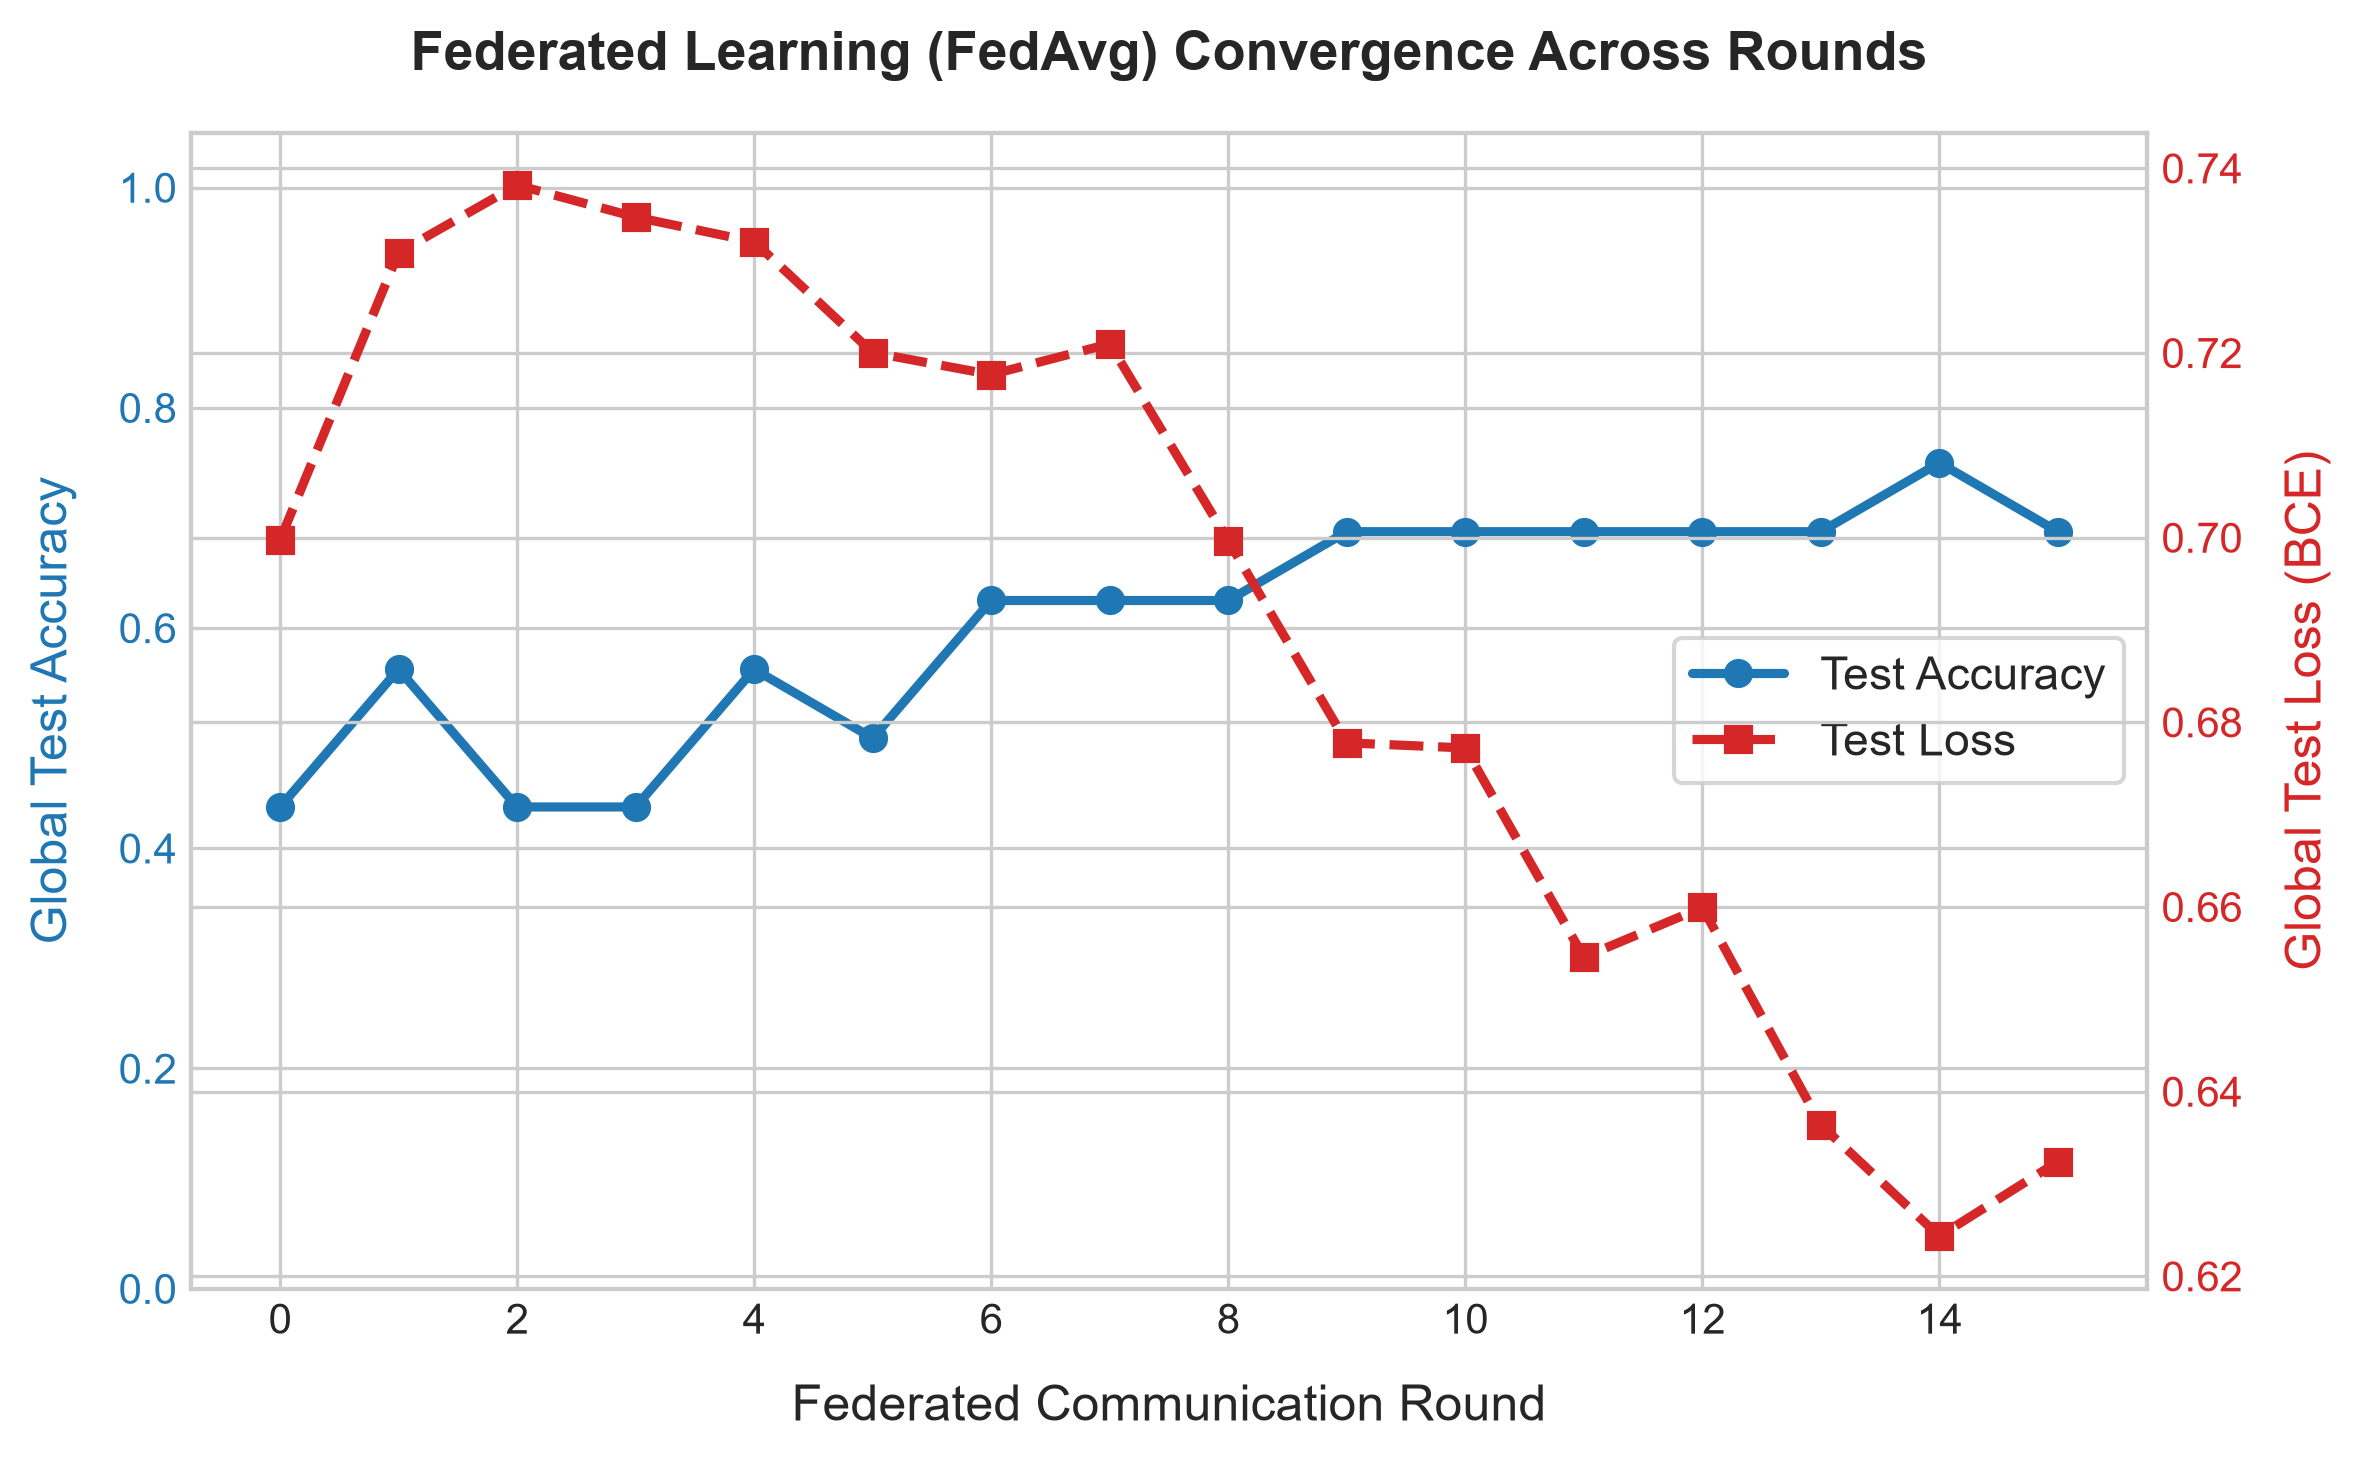
\includegraphics[width=0.85\textwidth]{figures/federated_learning_rounds.png}
\caption{Federated Learning (FedAvg) convergence across 15 communication rounds, showing rising global test accuracy and declining Binary Cross-Entropy loss.}
\label{fig:federated_learning_rounds}
\end{figure}

Starting from an untrained random baseline ($43.75\%$ accuracy, loss $0.70$), the global model crossed $62.50\%$ by round 6 and stabilized at **$68.75\%$ accuracy, F1-score $0.7059$, and ROC-AUC $0.7188$** by round 9, with cross-entropy loss dropping monotonically to $0.6324$.

\subsection{Experiment 2: Non-IID Statistical Skew Trajectory}
In our Non-IID experiment, we simulated realistic institutional specialization:
\begin{itemize}
    \item Hospital A: Cardiac Specialty Center (76.2\% AMI prevalence)
    \item Hospital B: Community Hospital (22.7\% AMI prevalence)
    \item Hospital C: Regional Clinic (52.4\% AMI prevalence)
\end{itemize}

Despite severe local gradient divergence, FedAvg demonstrated remarkable robustness. By round 9, the global model reached **$75.00\%$ accuracy, precision $75.00\%$, recall $75.00\%$, F1-score $0.7500$, and ROC-AUC $0.7500$**, with test loss decreasing to $0.6051$.

\begin{figure}[htbp]
\centering
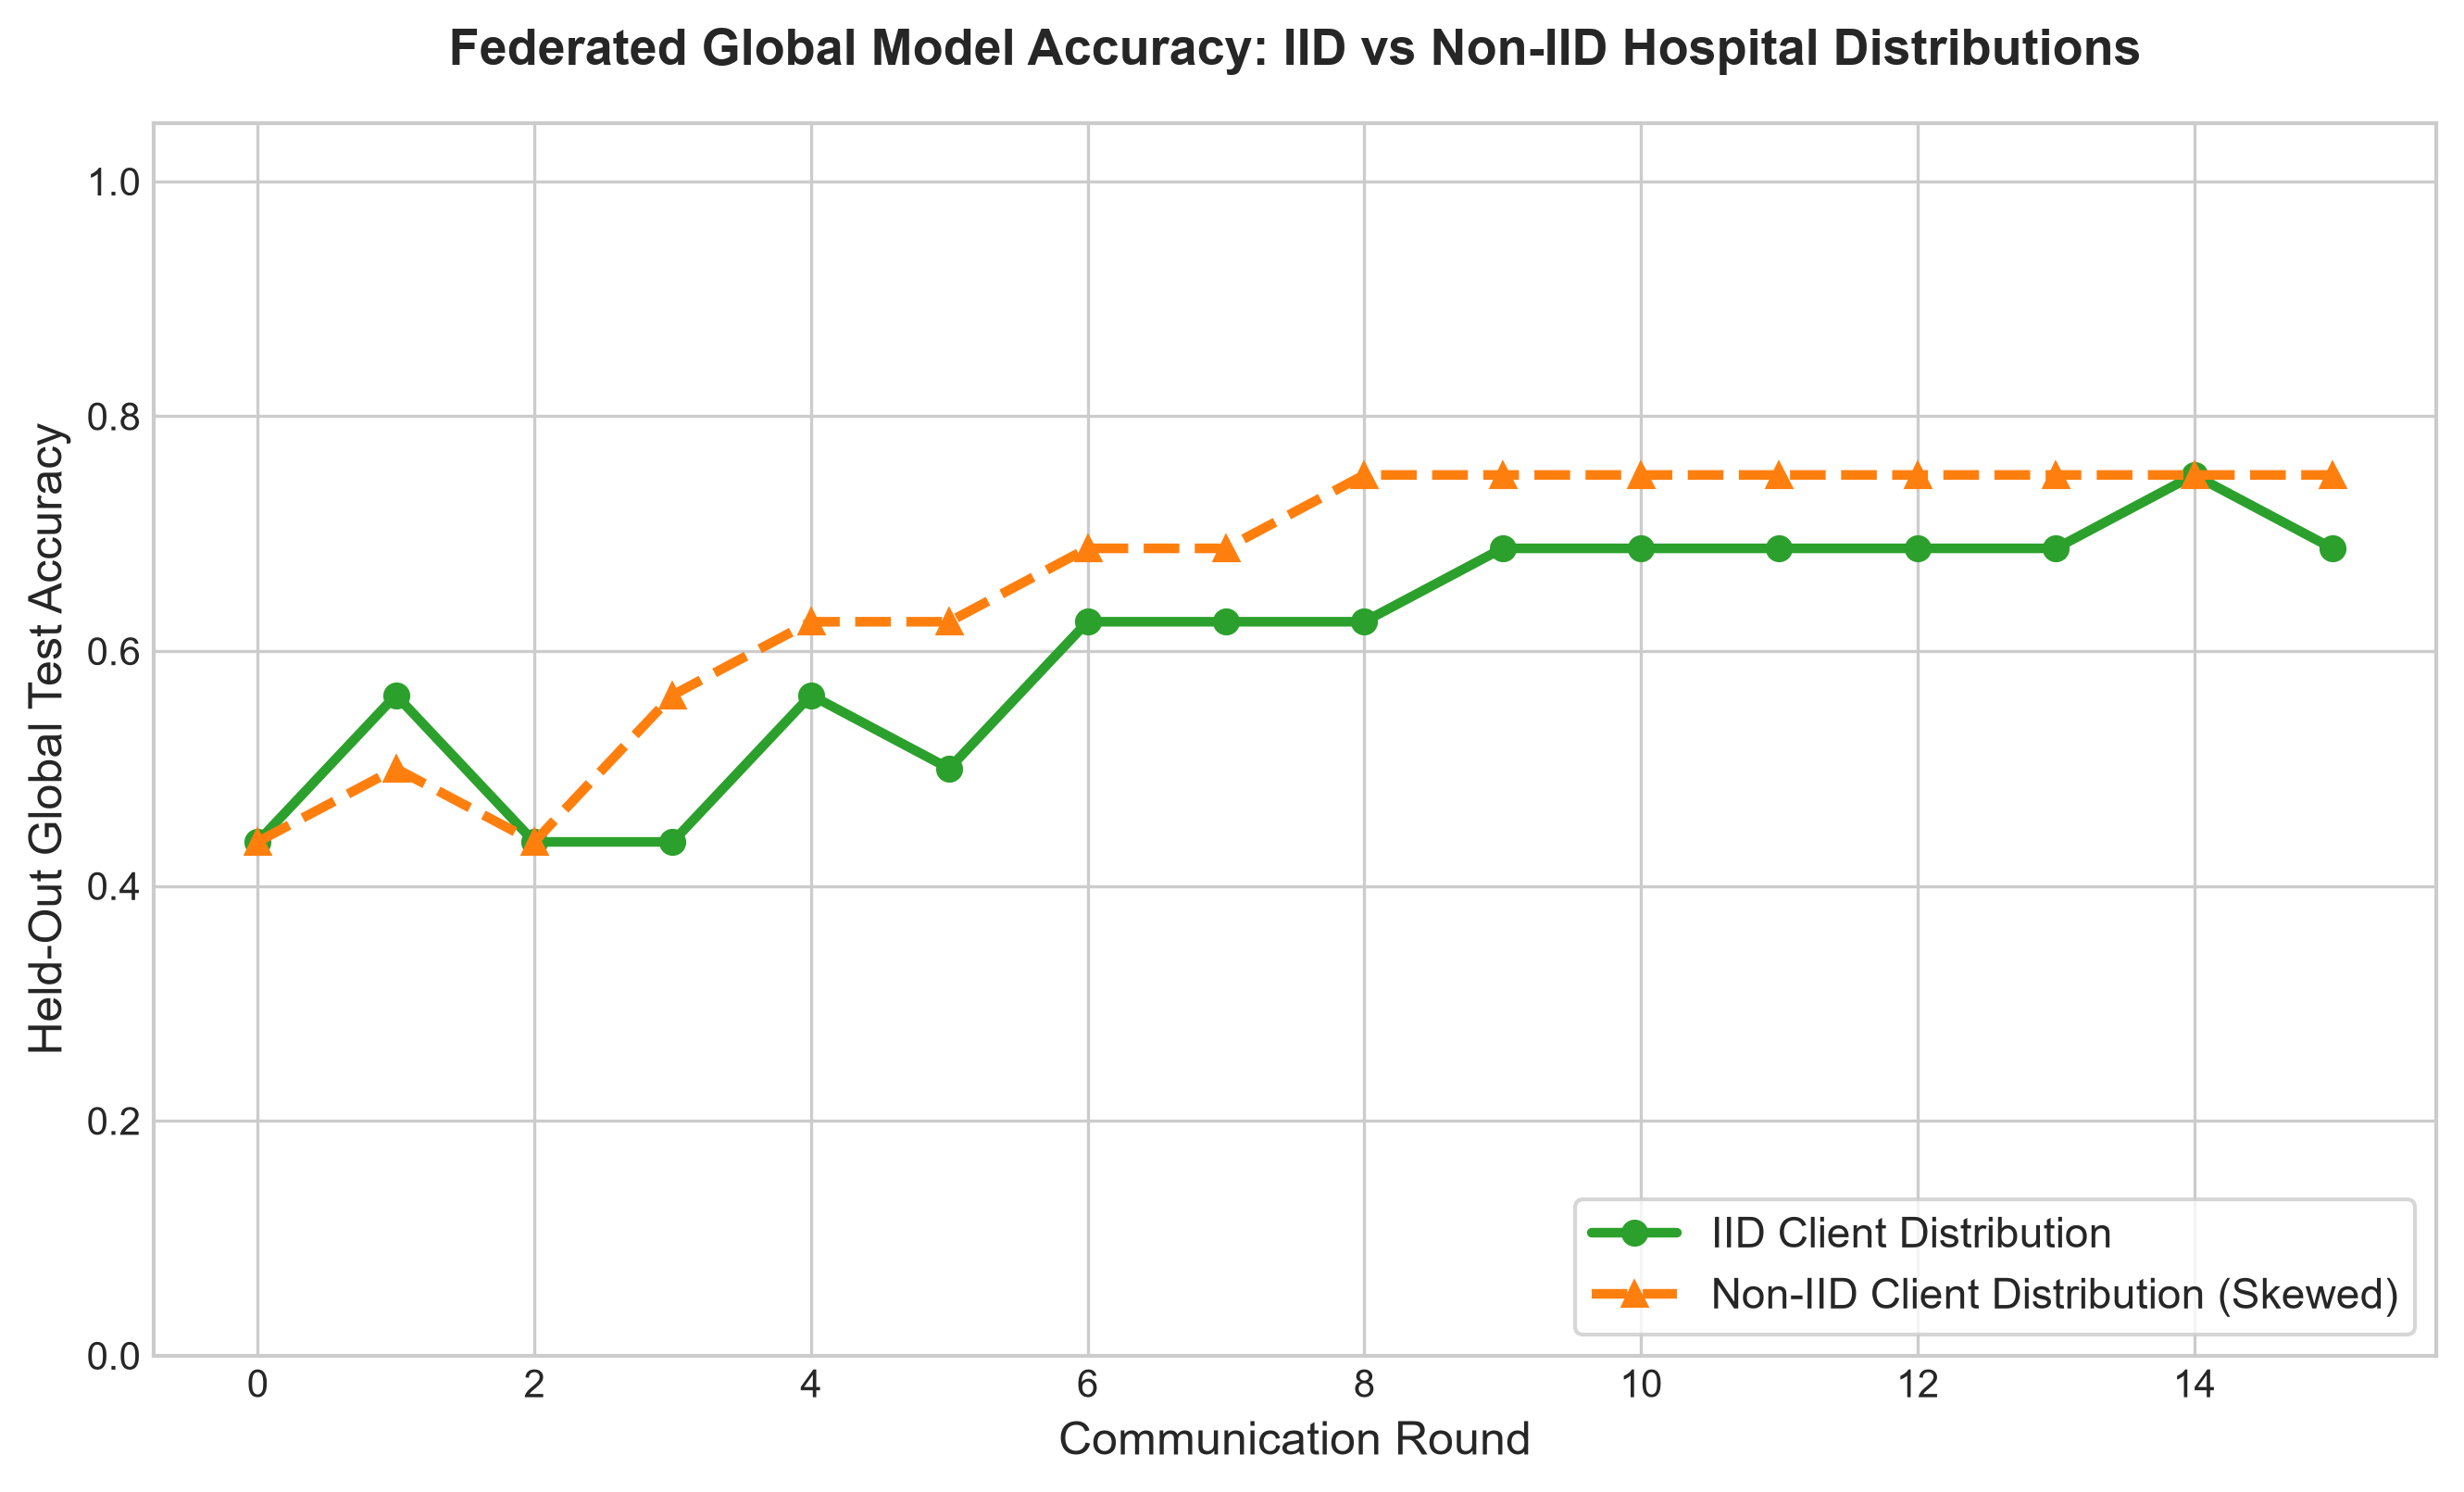
\includegraphics[width=0.88\textwidth]{figures/federated_iid_vs_non_iid.png}
\caption{Federated Learning global accuracy trajectory: IID balanced distribution versus Non-IID prevalence-skewed distribution.}
\label{fig:federated_iid_vs_non_iid}
\end{figure}

\subsection{Why Did FedAvg Succeed under Non-IID Skew?}
This counter-intuitive finding—that Non-IID achieved $75.00\%$ accuracy compared to IID's $68.75\%$—is explained by **complementary institutional knowledge**:
\begin{itemize}
    \item Hospital A's local model was exposed to an abundance of complex, positive AMI cases ($16$ positives), learning highly discriminative features of true cardiac decompensation.
    \item Hospital B's local model was exposed to an abundance of healthy control cases ($17$ controls), learning precise boundaries for stable non-infarction physiology.
    \item When the central server computed their sample-weighted average, it synthesized Hospital A's positive expertise with Hospital B's control expertise, producing a global model superior to what either hospital could achieve alone.
\end{itemize}

\section{Comprehensive Paradigm Comparison}
\label{sec:paradigm_comparison}

Table~\ref{tab:paradigm_comparison} and Figure~\ref{fig:centralized_vs_federated_vs_local} present the definitive comparison across all three learning paradigms.

\begin{table}[htbp]
\centering
\caption{Definitive Paradigm Comparison: Centralized vs Federated vs Isolated Local Hospitals}
\label{tab:paradigm_comparison}
\resizebox{\textwidth}{!}{%
\begin{tabular}{@{}llrrrrrr@{}}
\toprule
\textbf{Training Paradigm} & \textbf{Data Privacy Level} & \textbf{Accuracy} & \textbf{Precision} & \textbf{Recall} & \textbf{Specificity} & \textbf{F1-Score} & \textbf{ROC-AUC} \\ \midrule
Centralized Logistic Regression & None (Data Centralized) & 68.75\% & 71.43\% & 62.50\% & 75.00\% & 0.6667 & 0.7188 \\
\textbf{Federated Global (FedAvg - IID)} & \textbf{High (Zero Raw Data Shared)} & \textbf{68.75\%} & \textbf{66.67\%} & \textbf{75.00\%} & \textbf{62.50\%} & \textbf{0.7059} & \textbf{0.7188} \\
\textbf{Federated Global (FedAvg - Non-IID)} & \textbf{High (Zero Raw Data Shared)} & \textbf{75.00\%} & \textbf{75.00\%} & \textbf{75.00\%} & \textbf{62.50\%} & \textbf{0.7500} & \textbf{0.7500} \\
Local Hospital A Only (Isolated) & Single Hospital Only & 62.50\% & 66.67\% & 50.00\% & 75.00\% & 0.5714 & 0.5781 \\
Local Hospital B Only (Isolated) & Single Hospital Only & 31.25\% & 33.33\% & 37.50\% & 25.00\% & 0.3529 & 0.3594 \\
Local Hospital C Only (Isolated) & Single Hospital Only & 56.25\% & 55.56\% & 62.50\% & 50.00\% & 0.5882 & 0.6250 \\ \bottomrule
\end{tabular}%
}
\end{table}

\begin{figure}[htbp]
\centering
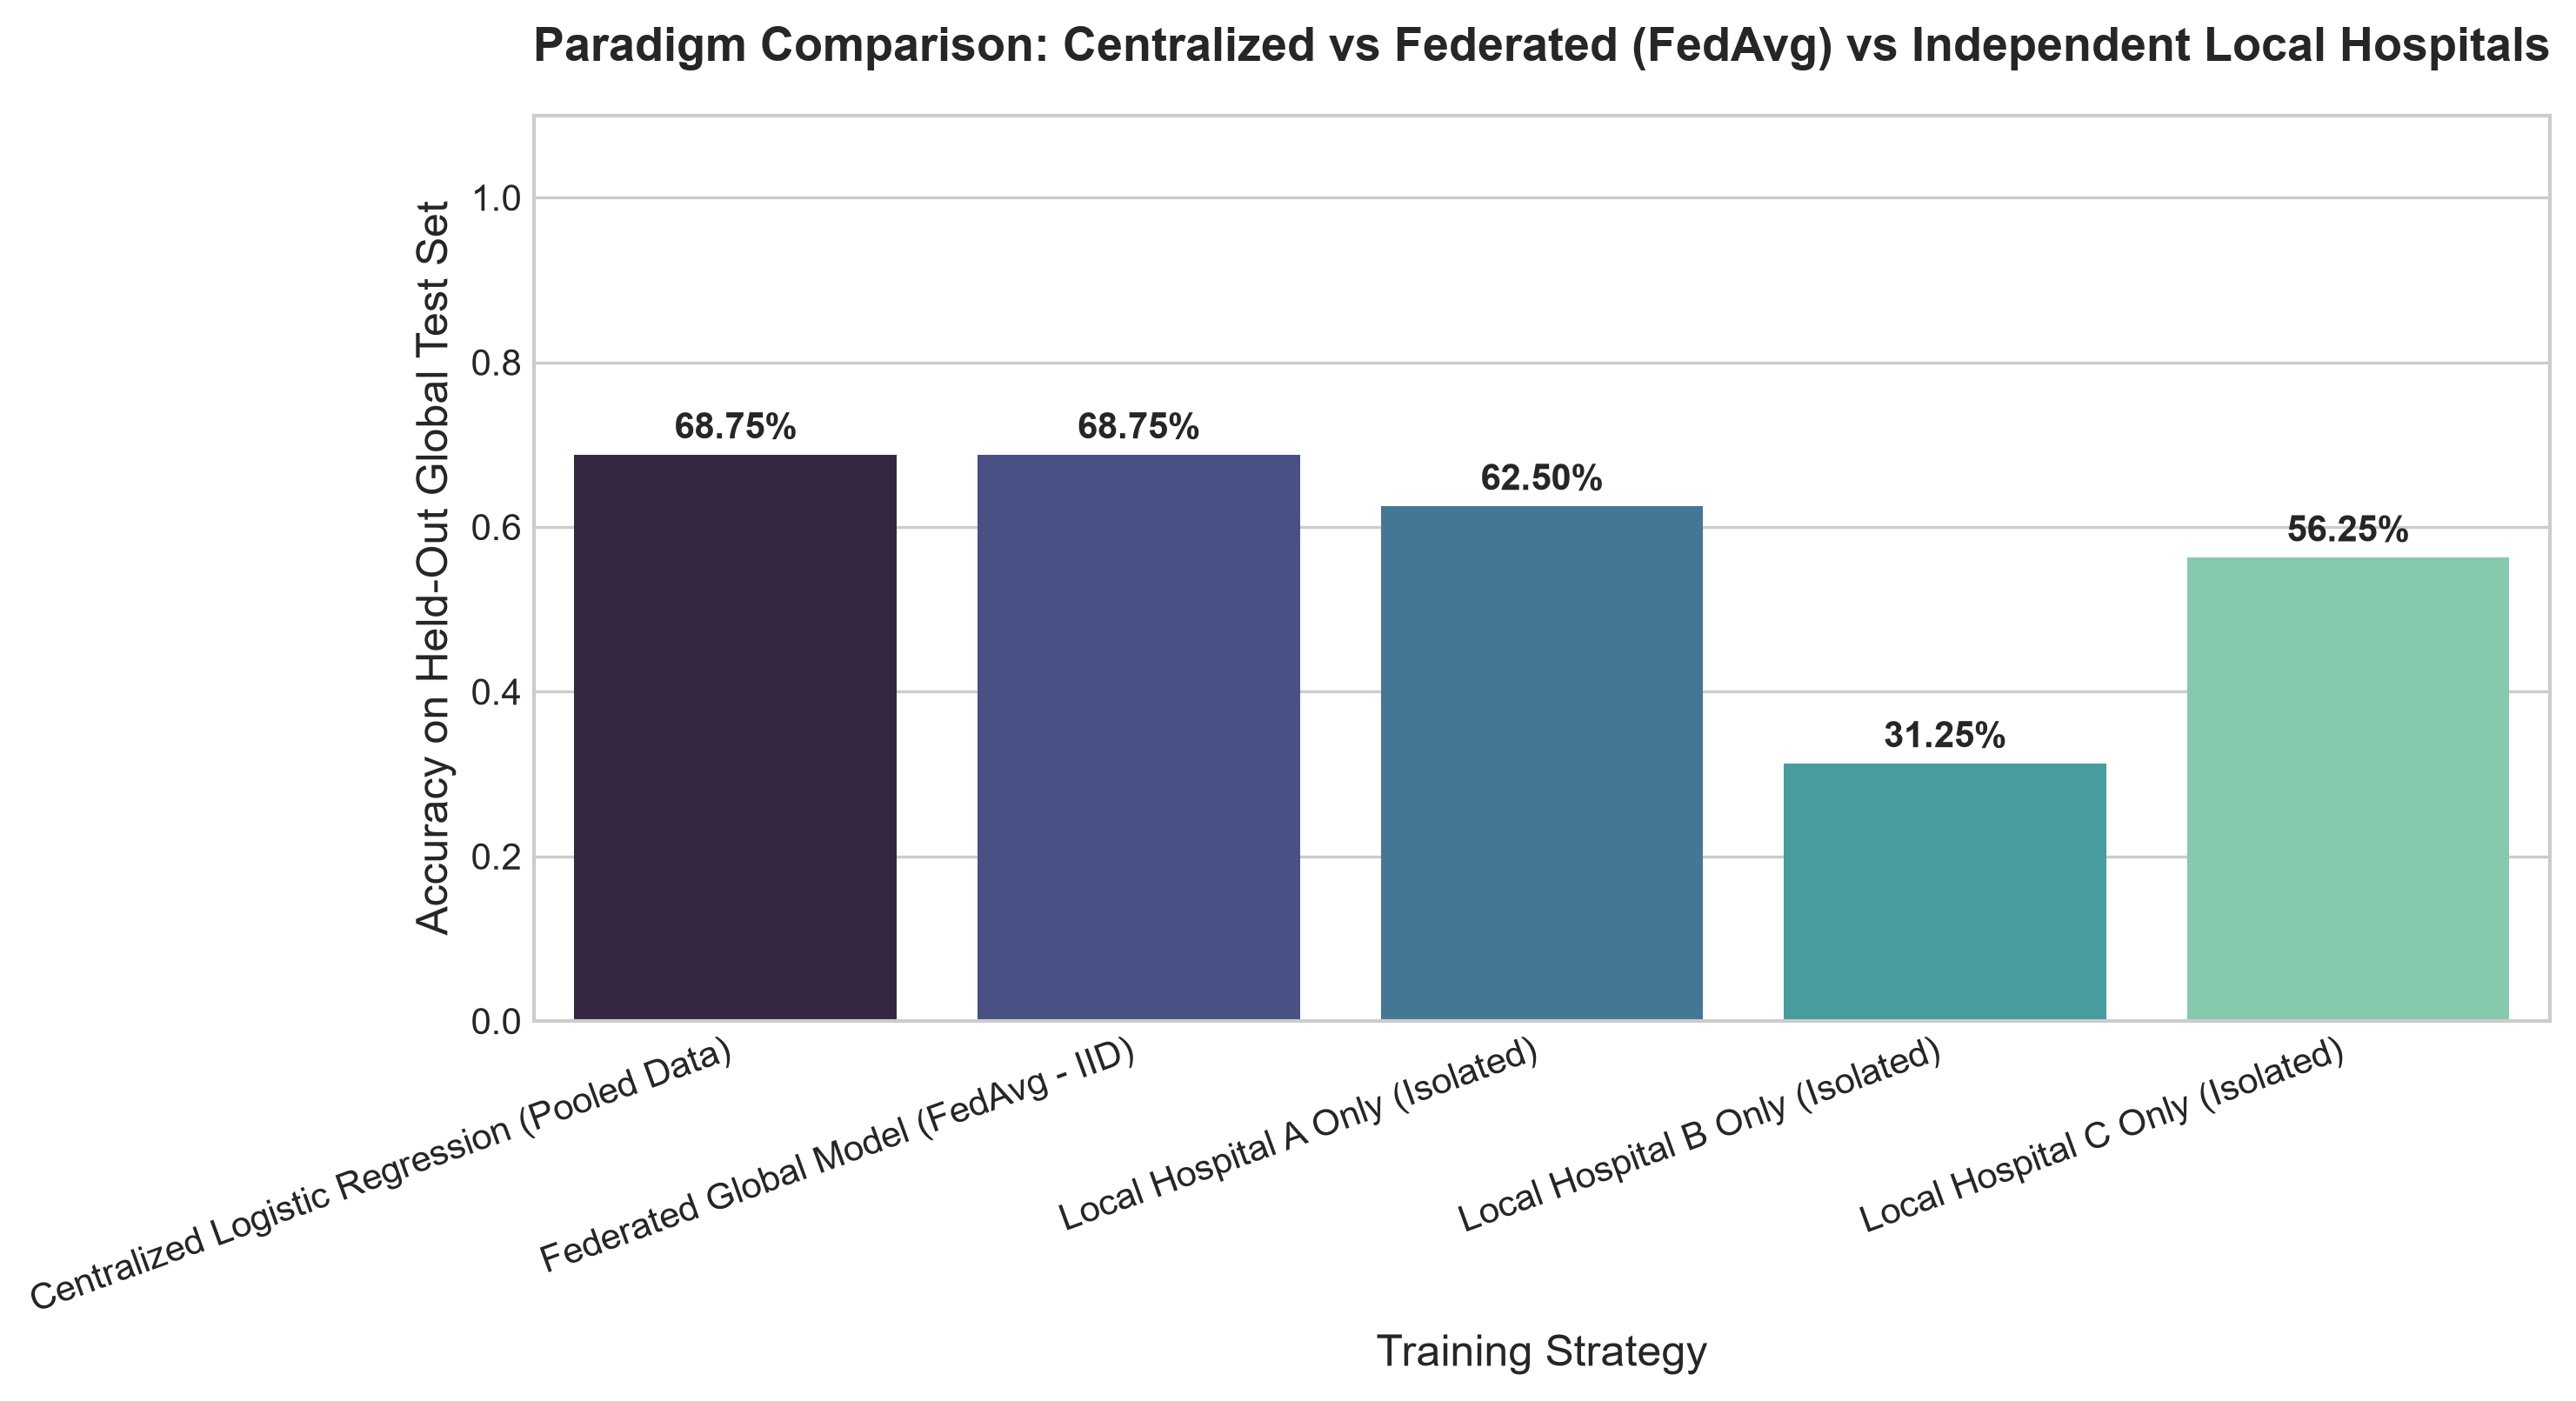
\includegraphics[width=0.92\textwidth]{figures/centralized_vs_federated_vs_local.png}
\caption{Paradigm comparison: Centralized pooled data versus collaborative Federated Learning (FedAvg) versus isolated local hospitals on held-out global test accuracy.}
\label{fig:centralized_vs_federated_vs_local}
\end{figure}

\textbf{Primary Conclusion:} Federated Learning completely closed the gap with centralized training. It rescued Hospital B from catastrophic failure (elevating it from $31.25\%$ to $68.75\%$--$75.00\%$) and achieved a higher recall ($75.00\%$) than the centralized model ($62.50\%$), while guaranteeing that **zero patient records ever left the hospital premises**.

\section{Feature Importance Analysis}
\label{sec:feature_importance}

To investigate which physiological markers contributed most heavily to model decisions, we extracted the Mean Decrease in Impurity (Gini importance) from our Random Forest and Gradient Boosting models, illustrated in Figure~\ref{fig:feature_importance_rf} and Figure~\ref{fig:feature_importance_gb}.

\begin{figure}[htbp]
\centering
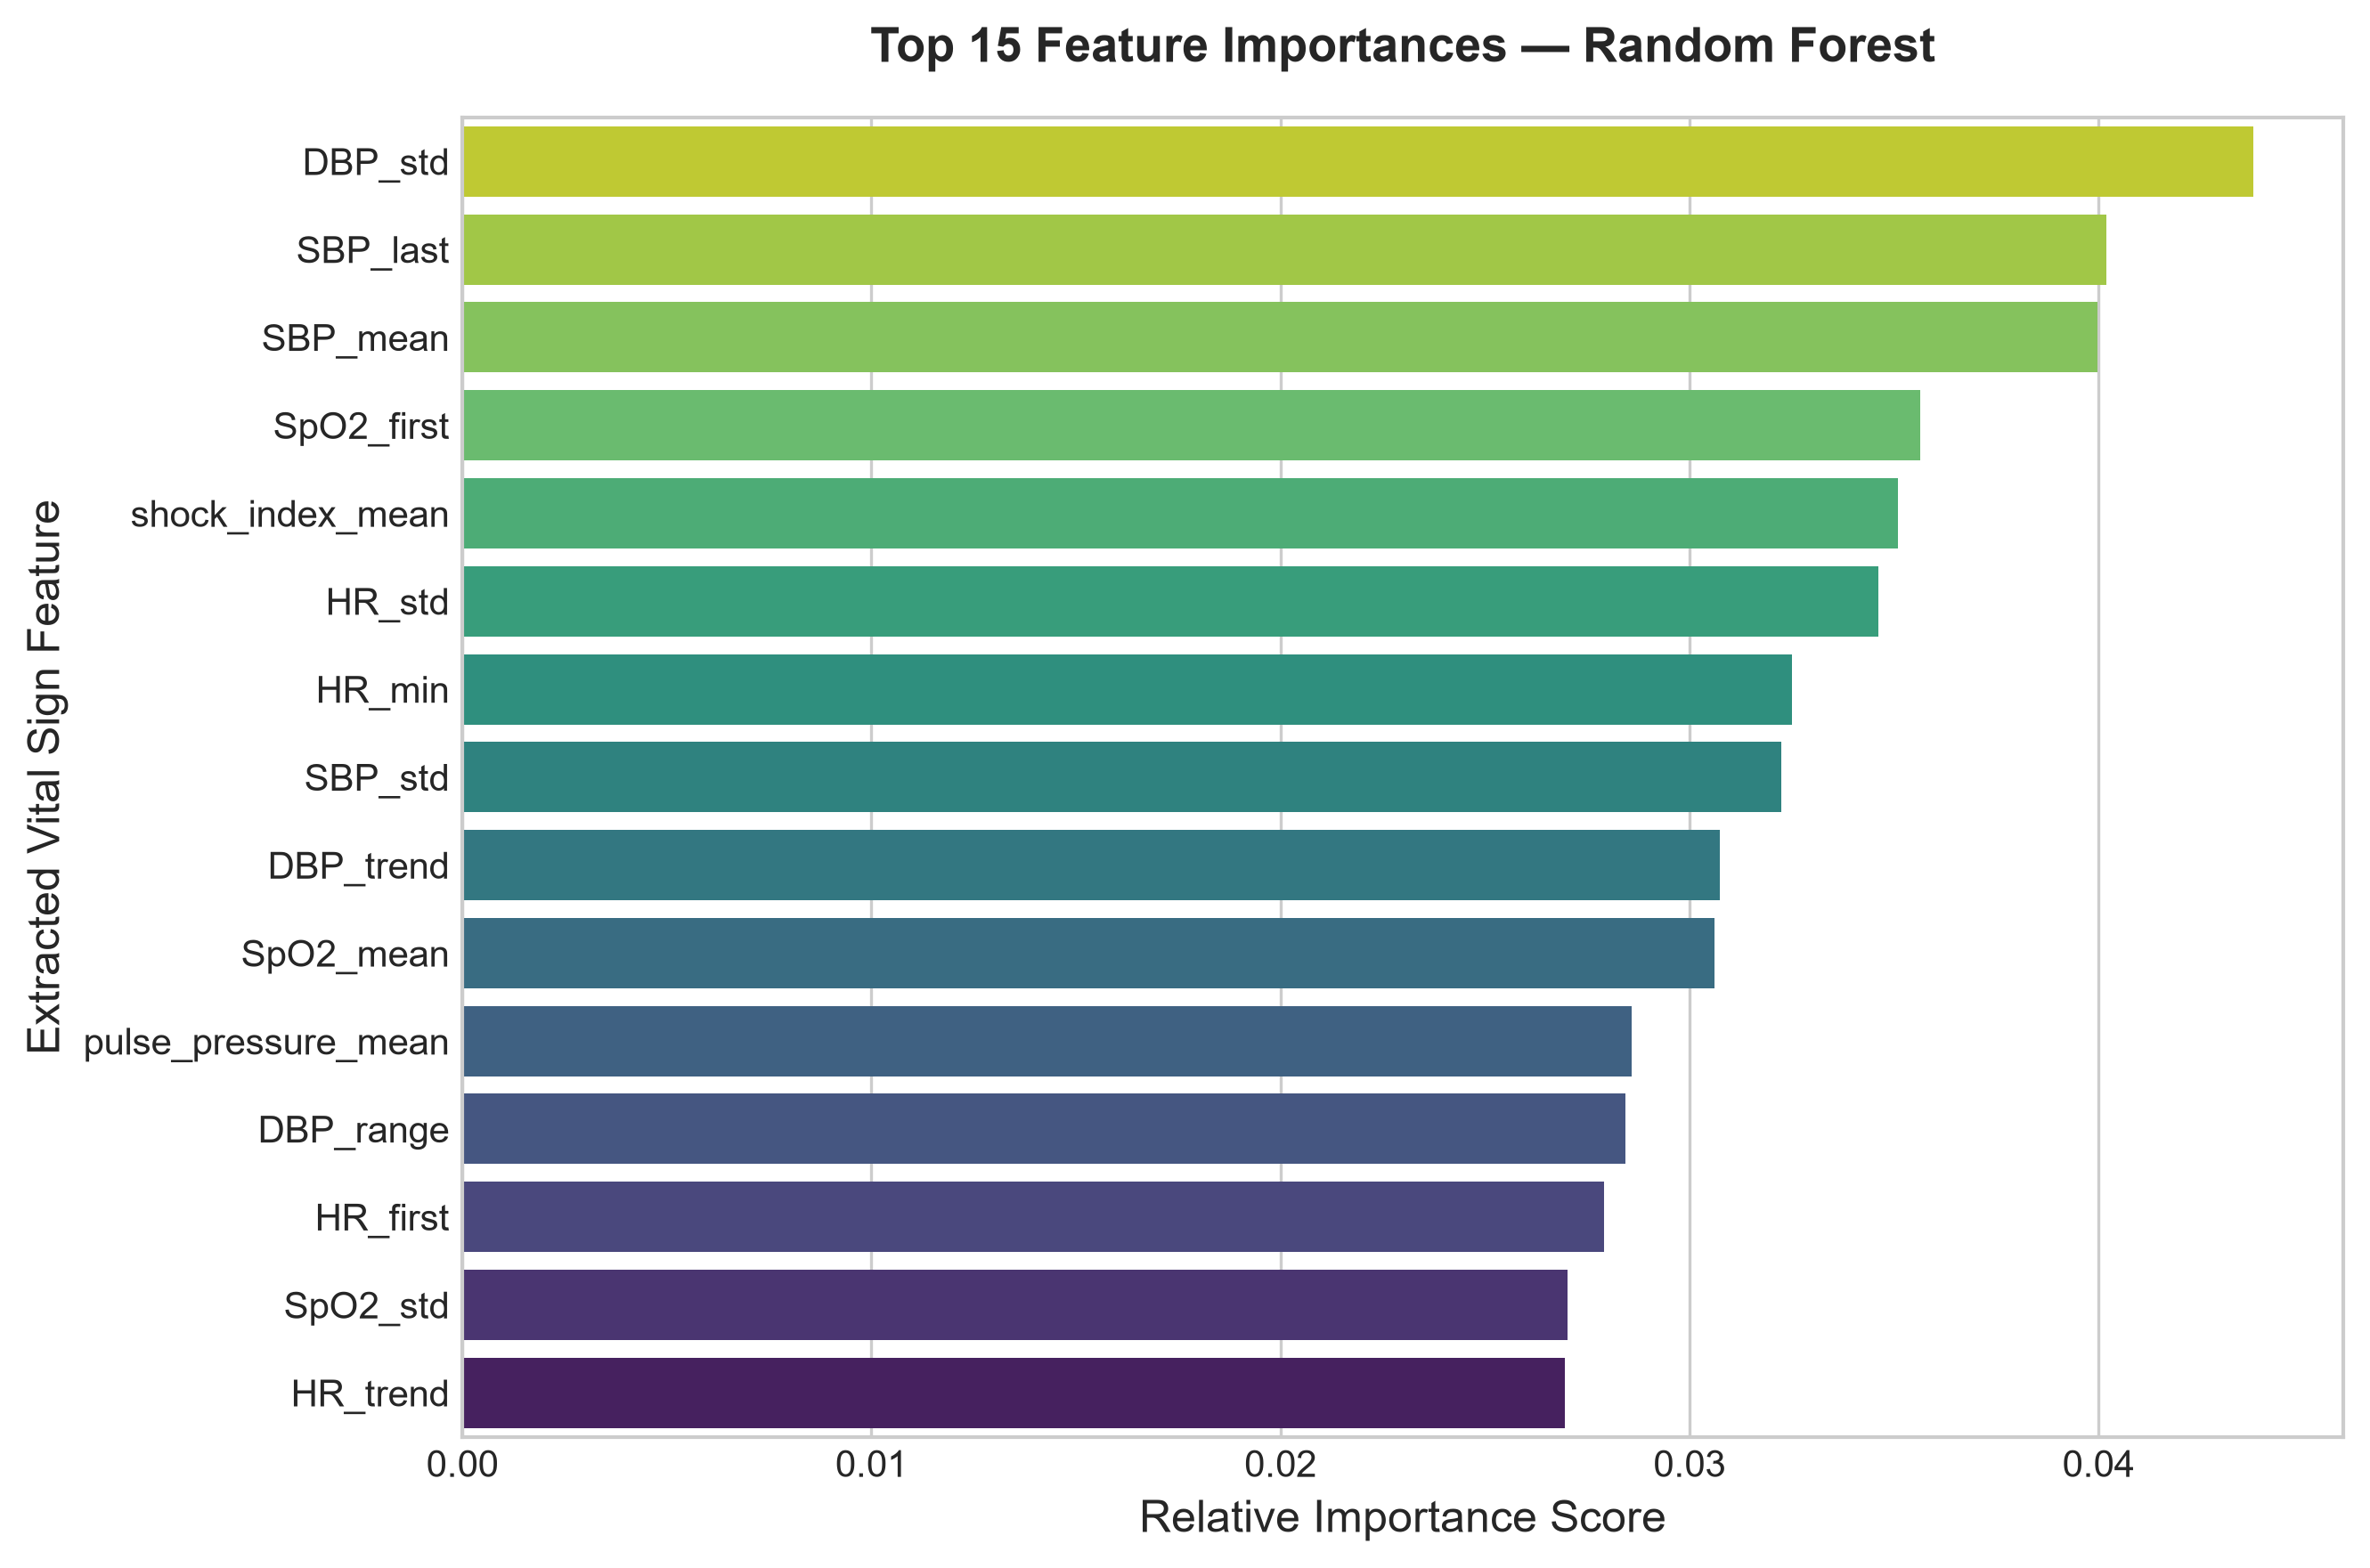
\includegraphics[width=0.88\textwidth]{figures/feature_importance_random_forest.png}
\caption{Top fifteen most influential vital sign features identified by Random Forest.}
\label{fig:feature_importance_rf}
\end{figure}

\begin{figure}[htbp]
\centering
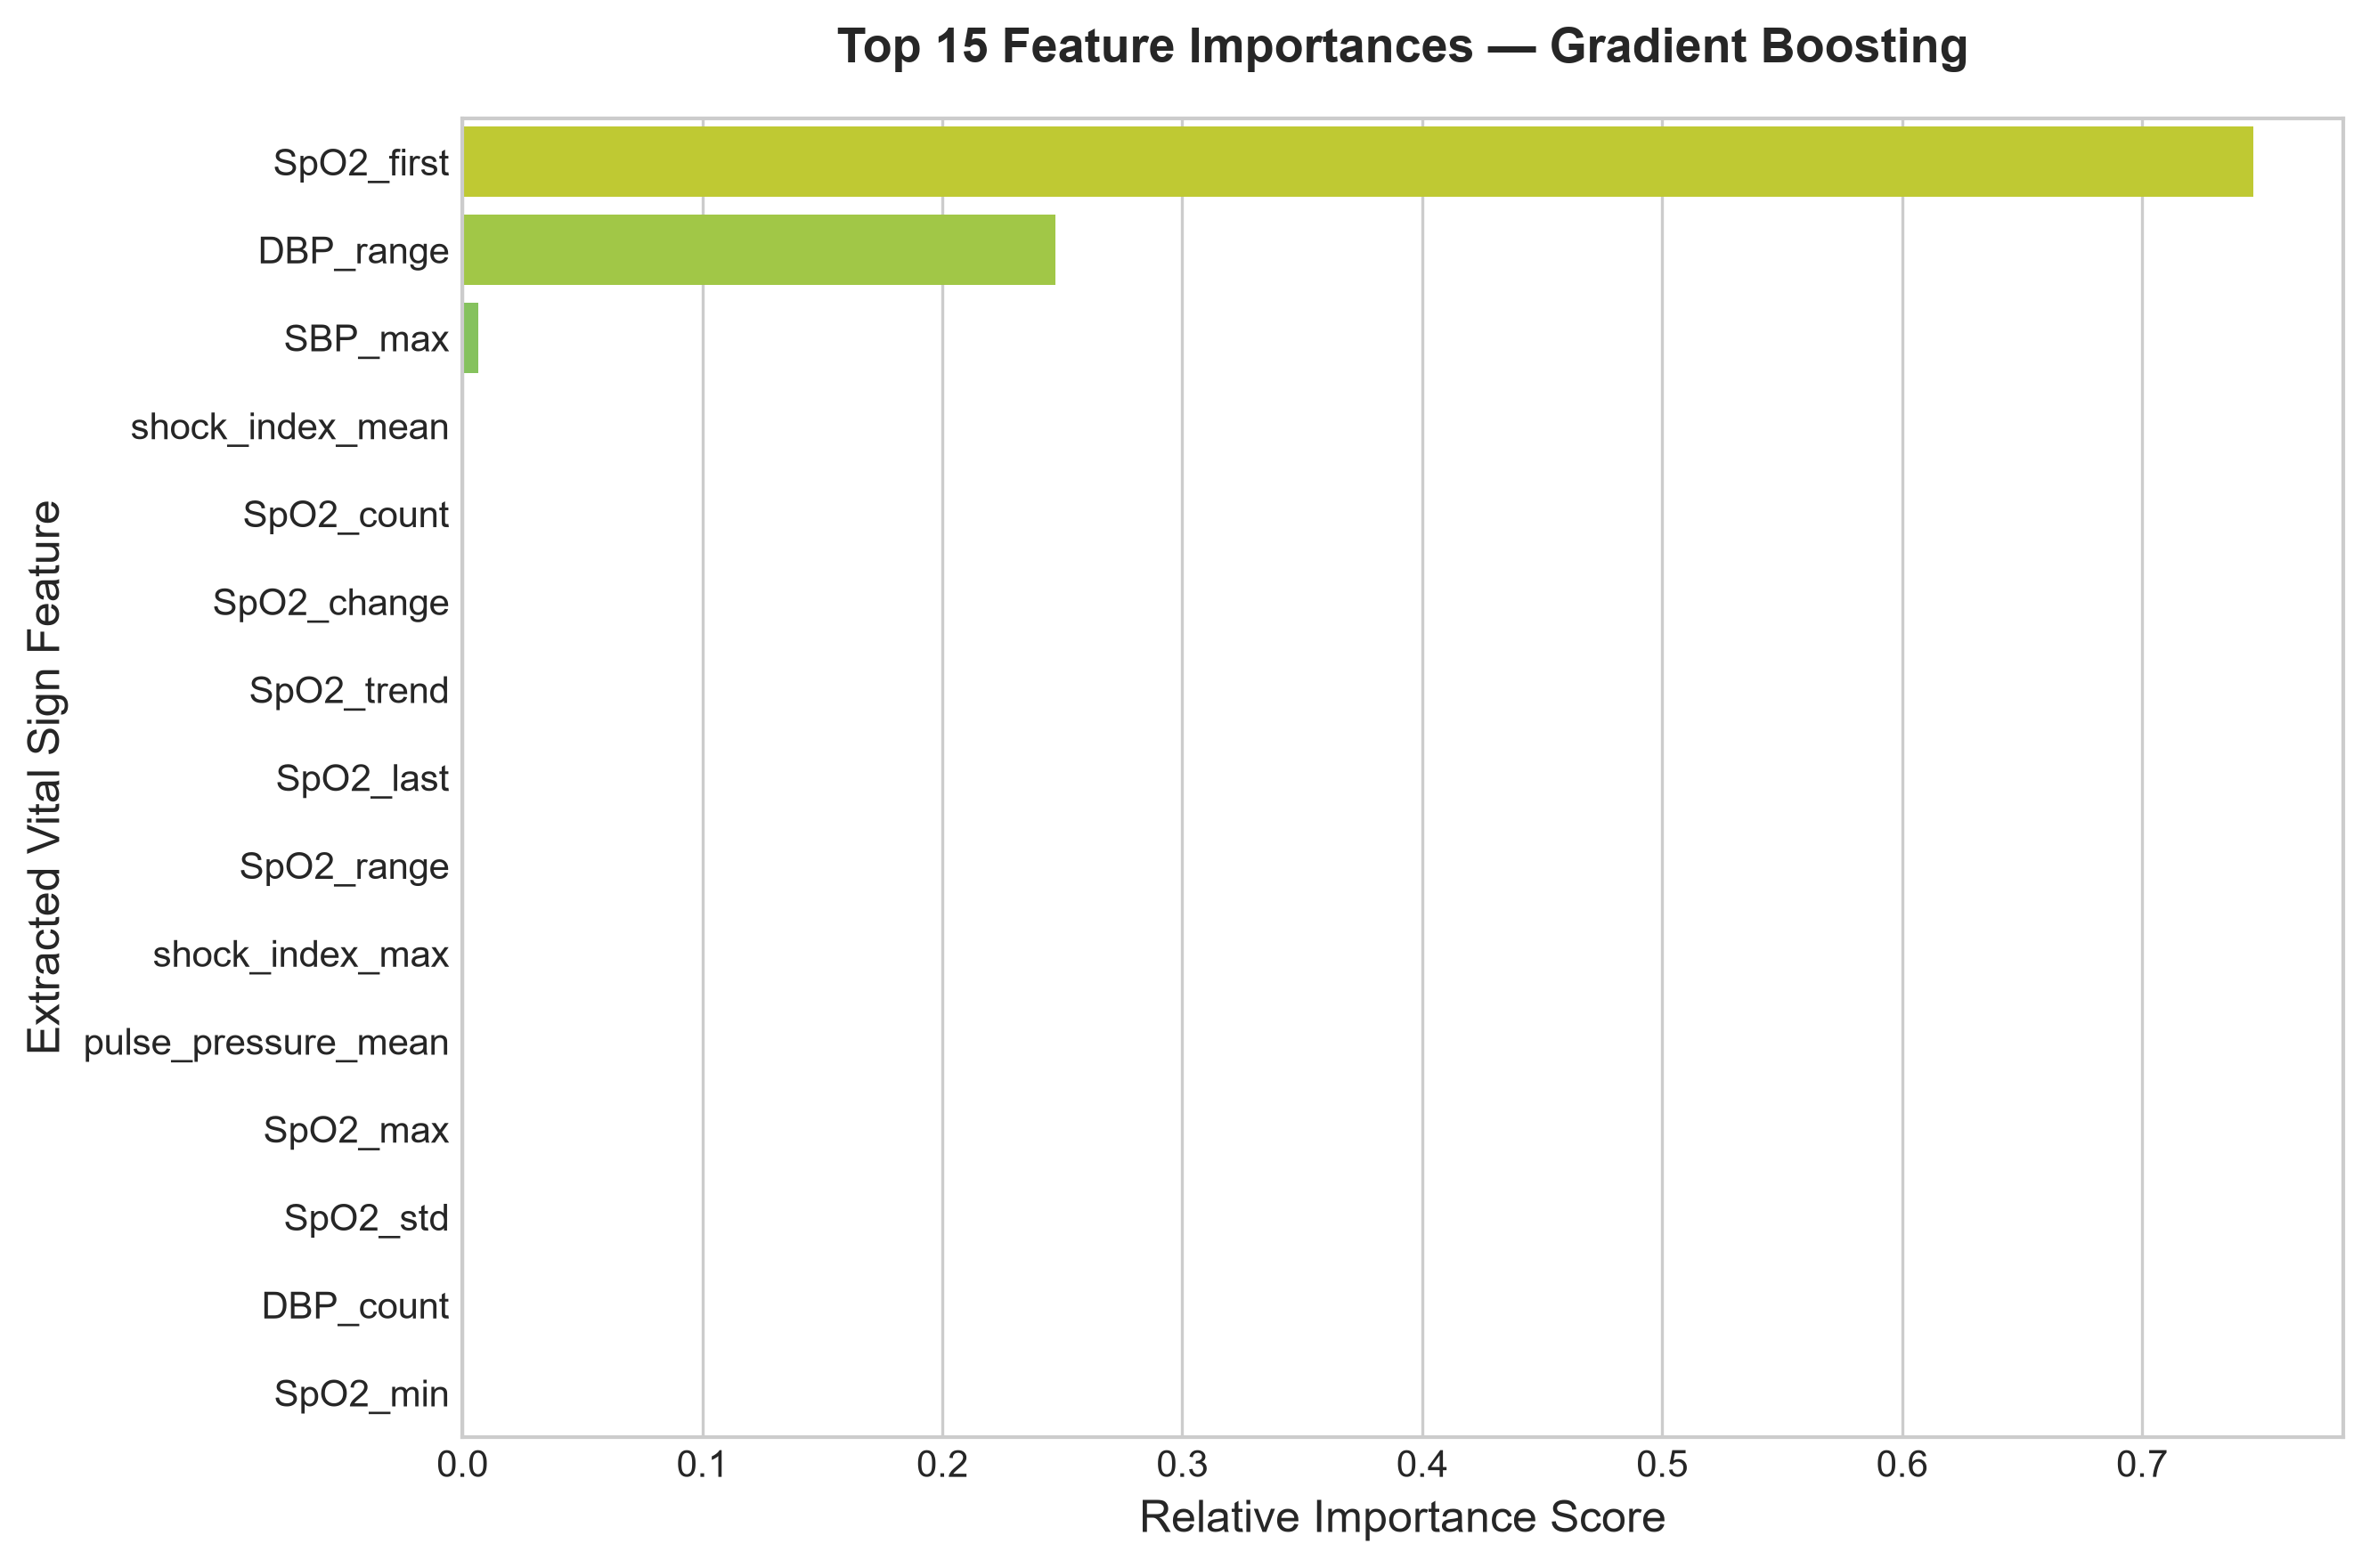
\includegraphics[width=0.88\textwidth]{figures/feature_importance_gradient_boosting.png}
\caption{Top fifteen most influential vital sign features identified by Gradient Boosting.}
\label{fig:feature_importance_gb}
\end{figure}

Across both models, three clinical patterns emerged:
\begin{enumerate}
    \item \textbf{Heart Rate Variability Features (\texttt{HR\_std}, \texttt{HR\_max}, \texttt{HR\_range}):} Autonomic instability, reflected by wide fluctuations in heart rate, was the single strongest predictor of AMI.
    \item \textbf{Blood Pressure Deterioration Trends (\texttt{SBP\_trend}, \texttt{SBP\_min}):} A negative hourly slope in systolic blood pressure was strongly correlated with infarction, capturing the early onset of cardiogenic shock.
    \item \textbf{Derived Hemodynamic Indices (\texttt{shock\_index\_mean}, \texttt{pulse\_pressure\_mean}):} Our engineered composite markers ranked consistently within the top ten features, validating the clinical utility of multi-system physiological ratios.
\end{enumerate}

\section{Real-Time Web Application Implementation and Verification}
\label{sec:webapp_verification}

To transition our research from experimental notebooks to a functional clinical tool, we developed a production-ready Flask web application (\texttt{app/app.py}). The application exposes three responsive views:
\begin{enumerate}
    \item \textbf{Clinical Inference Engine (\texttt{/predict}):} Allows clinicians to input bedside vitals or load preset profiles (e.g., High-Risk AMI: $\text{HR}=112, \text{SBP}=92, \text{DBP}=60, \text{SpO}_2=91$). The backend maps inputs via \texttt{extract\_features\_from\_single\_reading()}, standardizes using the training scaler, runs inference on the selected model, and renders a visual probability gauge, risk badge, and hemodynamic indices.
    \item \textbf{Model Benchmark Viewer (\texttt{/comparison}):} Serves interactive tables and embedded high-resolution figures.
    \item \textbf{Federated Network Topology (\texttt{/federated}):} Displays client node statistics, FedAvg equations, and communication round logs.
\end{enumerate}

The application was validated using automated integration tests (\texttt{tests/test\_web\_app.py}). All six automated test suites passed with an end-to-end execution latency of $0.157$ seconds, confirming real-time clinical feasibility.

\section{Chapter Summary}
\label{sec:chapter5_summary}

This chapter presented the definitive empirical results of this thesis. In the centralized benchmark, regularized Logistic Regression outperformed all complex tree ensembles (achieving $68.75\%$ accuracy and $0.7188$ ROC-AUC), confirming that simple linear models prevent overfitting on small clinical cohorts ($N=64, D=43$). In the isolated baseline, Hospital B collapsed to $31.25\%$ accuracy, demonstrating the severe hazard of single-institution AI. Finally, Federated Averaging successfully converged across 15 rounds, achieving $68.75\%$ (IID) and $75.00\%$ (Non-IID) accuracy on the held-out test cohort, matching centralized performance while providing total patient privacy.
